%HEADER
%%%%%%%%%%%%%%%%%%%%%%%%%%%%%%%%%%%%%%%%%%%%%%%%%%%%%%%%%%%%
\documentclass[a4paper, %Format
		11pt, %Font size
		headsepline,
%toc - table of content
		toc=listof, %Include TOC
		toc=listofnumbered, %Number TOC
		toc=bibliography, %Literaturverzeichnis ins TOC
		toc=bibliographynumbered, %Literaturverzeichnis im TOC nummerieren
		]{scrreprt} %Doc class[Optionen]

%Bibliography
\usepackage[sorting=none]{biblatex}
\bibliography{literatur.bib} %Literaturverzeichnis

%GEOMETRIE UND AUSSEHEN
\usepackage[left=35mm,right=30mm,top=15mm,bottom=25mm]{geometry} %Set text geometry
\linespread{1.3}
\setlength{\parindent}{0pt} %dissable first line spacing
\usepackage{microtype} %automatically adjust distance between letters

\usepackage{color} %Colorpackage
\definecolor{lightgrey}{rgb}{0.97,0.97,0.97} %definition von "lightgrey"
\usepackage[skip=2pt,font=footnotesize]{caption}


%SONDERZEICHEN UND DEUTSCHE ÜBERSETZUNG
%\usepackage{ucs}
\usepackage[utf8]{inputenc} %UTF-8 
\usepackage[ngerman, english]{babel}
\usepackage[text]{}

%Tables
\usepackage{booktabs} %extended table options
\usepackage{multirow} %tableelements over multiple rows
\usepackage{csvsimple}

%Graphs
\usepackage{graphicx} %Insert graphics
\usepackage{subfig}


%Sourcecode
\usepackage{scrhack}
\usepackage{listings} %u.a. Darstellen von Sourcecode
\renewcommand\lstlistingname{Quelltext} %Übersetzung/Umbenennung von "listing" in "Quelltext"
\renewcommand\lstlistlistingname{Quelltextverzeichnis} %Übersetzung von "Quelltextverzeichnis"
%Darstellungsoptionen von Sourcecode
\lstset{numbers=left, numberstyle=\tiny, stepnumber=1, captionpos=b, backgroundcolor=\color{lightgrey}, breaklines=true; float=htbp;} 

%TOC
\usepackage{titletoc}
%\dottedcontents{chapter}[1.5em]{ }{2.3em}{1pc}

%Footnotes
\usepackage{chngcntr}
\counterwithout{footnote}{chapter} %durchgehende, kapitelübergreifende Nummerierung
\setlength{\skip\footins}{10mm} % bestimmt den Abstand zwischen der Grenzlinie der Fußnoten und dem Fließtext.


%Head and Bottom line
\usepackage{scrpage2} %Paket für Kopf/Fusszeilen
%\renewcommand*{\chapterpagestyle}{scrheadings} %Seite eines Kapitelbeginn: Linie in Kopfzeile,

%Literature
%\usepackage{cite} %Paket für Literaturverweise

%HYPERLINKS
\usepackage{url} %Erleichtert Darstellung von URL (viele Sonderzeichen)
\usepackage[pdftex]{hyperref} %Erstellt Hyperlinks im PDF
% Nach "hyperref" sollten keine weiteren Pakete eingebunden werden,
% da "hyperref" gewisse Befehle umdefiniert.








%%%%%%%%%%%%%%%%%%%%%%%%%%%%%%%%%%%%%%%%%%%%%%%%%%%%%%%%%%%%
%DOKUMENT
\begin{document}

\clearscrheadfoot %löscht bisherige Kopf-Fusszeilen Definitionen
\setheadsepline{0pt} %Definition der Linienstärke in der Kopfzeile, hier 0

\startcontents[main] % Start TOC

\thispagestyle{empty}
\begin{titlepage}

\center
\includegraphics[width=70mm]{Pictures/Logo_HSAA}

\vspace*{8mm} %vertikaler Abstand von 10mm
\begin{center} %Text zentriert
	
	\Huge\center\textbf{Development and Simulation of an Autonomous Navigation for Mobile Robotic Platforms}\\ %Große Schrift, Fettschrift
	\vspace*{11mm}
	\Large{by}\\
	\Large{Tristan Schwörer}\\
	\Large{Matriculation number: 71336}\\
	
	\vspace*{11mm}
	
	\Large{A bachelor thesis submitted in fulfillment of the}\\
	\Large{requirements for the degree of the}\\
	
	\vspace*{11mm}
	
	\Large{Bachelor of Engineering (B. Eng.)}\\
	\Large{in mechatronics}\\
	\Large{at Aalen University}\\
	
	\vspace*{11mm}
	
	\Large{Supervisor:}\\
	\Large{Prof. Dr. Stefan Hörmann (Aalen University)}\\
	
	\vspace*{11mm}
	
	\Large{Submitted on:}\\
	\Large{April 13\textsuperscript{th}, 2021}\\
	\todo{Date!}
\end{center}
\end{titlepage}


%%Leerseite
\thispagestyle{empty}
\hspace{1mm}\\

\newpage
\pagenumbering{roman} %römische Seitenzahlen
\setcounter{page}{1} %Seitenzähler zurücksetzen

\thispagestyle{empty}
\chapter*{Preface}
\addcontentsline{toc}{chapter}{Preface}
\label{preface}

This bachelor thesis is part of the bachelor program in mechatronics at Aalen University and is supposed to take place in the \nth{7} Semester. It covers the theoretical and practical work between November \nth{2} 2020 and April \nth{13} 2021.\\

This work took place at the laboratory for mobile robotic systems of the faculty optics and mechatronics at aalen university and was completely independent of any other party and company.

\vspace*{25mm}

\begin{otherlanguage}{ngerman}
Diese Bachelorarbeit ist fester Bestandteil des Bachelorprogramms Mechatronik an der Hochschule Aalen und soll im siebten Semester statt finden. Die hier dokumentierte Arbeit wurde zwischen dem 2. November 2020 und dem 13. April 2021 realisiert.\\

Die praktische sowie die theoretische Arbeit fand im Labor für mobile Robotersysteme der Fakultät Optik und Mechatronik an der Hochschule Aalen statt und ist komplett unabhängig von jeglicher anderen dritten Partei oder Firma.
\end{otherlanguage} 

\thispagestyle{empty}
\chapter*{Abstract}
\addcontentsline{toc}{chapter}{Abstract}
\label{abstract}
This thesis covers the conceptual design, setup, development and testing of a software stack used for the autonomous navigation in an environment defined by the rules of the Carolo-Cup.\\

 The aim of this stack is lane following and obstacle avoidance based on sensory environmental data. This thesis extends work of the existing roadDetection package and is supposed to be used by the Carolo-Cup team of Aalen Univeristy in the future.\\
 
 The navigation is not supposed to be focussed only on Ackeramann steering, since the Carolo-Cup does not make restrictions to the steering type, other than at least one axle must be steerable, but ideally the stack should be as flexible as possible\cite{carolocup}.\\
 The laboratory for mobile robotic platforms at Aalen University owns multiple Parallax Arlo robots. To make future testing easier this type of robot is selected for this thesis.

 The robot used in this work does not satisfy the rules of the Carolo-Cup since it is to big and uses the wrong steering technique. Therefore the stack needs to be flexible in order to be adapted by the Carolo-Cup team.

The robot is equipped with a lidar sensor, a camera, wheel encoders and an IMU (Inertia Measurement Unit). The data of these sensors will be processed using existing ROS (Robot Operating System) packages as well as newly developed ones. The resulting data will be used by the navigation stack to determine the best route for the robot. This is done with the use of predictive algorithms.\\

For testing purposes and to make quick hardware changes possible, the robot and the entire system is simulated using the Gazebo simulation environment.\\

While maneuvering through the course the robot has to stay on the right lane of the road except when avoiding obstacles.

\thispagestyle{empty}
\chapter*{Kurzfassung}
\addcontentsline{toc}{chapter}{Kurzfassung}
\label{kurzfassung}

\begin{otherlanguage}{ngerman}
Um an dem Wettbewerb Carolo-Cup, ausgerichtet von der technischen Universität Braunschweig, teilzunehmen, sucht das Team der Hochschule Aalen nach einem neuen Navigationsalgorithmus für ihr Fahrzeug.\\

Da die Navigation ebenso wie die bereits vorhandene Spurerkennung auf ROS (robot operating system) basieren soll, wird der ROS navigation stack als Grundstruktur verwendet. Um Spurhalten, Spurwahl und Hindernissvermeidung zu gewährleisten, wurde die Standardkonfiguration des navigation stacks im Laufe dieser Arbeit modifiziert und durch weitere Funktionalität ergänzt. Die Ziele für die Navigation werden mit einen geschätzten zukünftigen Spurverlauf ermittelt, der auf der zuletzt erkannten Spur basiert.

Der vorgeschriebene Roboter verfügt über eine Kamera, einen Lidar-Sensor, eine IMU und Dreh-Encoder der Räder. Des Weiteren wird ein Differenzialantrieb verwendet.

Eine Simulation des Roboters, mitsamt der Umgebung wurde aufgebaut, um die Navigation zu testen. Dies ermöglichte auch schnelle und effiziente Änderungen des Roboters und der Umgebung.

Die Testergebnisse zeigen, das der navigation stack eine geeignete Grundstruktur für die Navigation des Carolo-Cup Fahrzeuges bietet.

Der gewählte Aufbau der Navigation ist eine vielversprechende Basis für das Carolo-Cup Team, da zukünftige Ergänzungen zum Fahrverhalten durch die flexible Struktur ermöglicht werden.
\end{otherlanguage}


\thispagestyle{empty}
\chapter*{Acknowledgement}
\addcontentsline{toc}{chapter}{Acknowledgement}
\label{acknowledgement}
At this point I would like to thank the following people who made my bachelor thesis possible and supported me during my time in Sweden:

\begin{itemize}
\item \textbf{Sabina Rebeggiani} for being a great supervisor during my time in Sweden. She taught me a lot of knowledge about surface metrology and the scientific of working. 
\item \textbf{Martin Bergman} for supervising me in the relationship with Volvo and teaching me about design and soft metrology.
\item \textbf{Lars B\aa \aa th} for supervising me with the optics and physics of the project.
\item \textbf{Ulrich Schmitt} for supervising me at Aalen University during my bachelor thesis.
\item \textbf{Rainer Börret} for supervising me at Aalen University during my bachelor thesis and making my studies abroad possible.
\item \textbf{Volvo Cars}, especially Ola Wagersten, Anna Larsson and Viktor Wadenvik for the bi-weekly meetings and the provided information about soft metrology and the quality control process at Volvo Cars.
\item \textbf{Tim Malmgren and Joakim Wahlberg} for always helping out with practical work and the machines in FabLAB.
\item \textbf{Lukas Ziegler} for his help during the last month of my thesis.
\end{itemize}

Last but not least I want to thank my family for their continuous support they have given me throughout my time in Sweden and my whole studies.

% Insert TOC
\renewcommand\contentsname{\huge Table of Contents}% Change TOC Name and size
\printcontents[main]{ }{0}{\section*{\contentsname}}
\newpage

%KOPF-/FUSSZEILE
\pagestyle{scrheadings} 
\clearscrheadfoot %löscht bisherige Kopf-Fusszeilen Definitionen
\automark[]{chapter} %[rechte Seite]{linke Seite}
\chead[]{\headmark} %oben mitte
\cfoot[\pagemark]{\pagemark} %Seitenzahlen auf [Seite des Kapitelbeginns]{den folgenden Seiten}
\setheadsepline{0.5pt} %Definition der Linienstärke in der Kopfzeile, hier 0,5

\newpage
\pagenumbering{arabic} %arabische Seitenzahlen
\setcounter{page}{1} %Seitenzähler zurücksetzen

\chapter{Introduction}
\label{introduction}
\todo{Abkürzungsverzeichniss}

When looking at the recent trends in the car industry, autonomous driving is probably one of the most important topics.\todo{lot of research like company xy article tesla?} Furthermore, this trend can also be seen in other industries  in which autonomous robots are used to simplify and accelerate production steps. 



The event ``Carolo-Cup''\todo{name consistency} hosted by the Technical University of Braunschweig offers a place for teams to compete against each other with their autonomous 1:10 model cars and therefore supports the development of the research field itself. This creates an incentive to participate to a lot of universities in Germany and beyond.\\
\todo{existing, goal and this work relations }

At the moment of the start of this work the existing part was solely the roadDetection developed by Prof. Dr.-Ing. Stefan Hörmann with the goal to use it in the Carolo-Cup. To use it, a software stack has to be build around it, that uses the data to navigate the robot on the course, the development of which is covered in this thesis.


The navigation of a mobile system from ground up includes a wide range of topics and problems, such as sensor data filtering and combination to generate a stable and reliable odometry, or path finding in an environment including obstacles with respect to the dynamics of the robot.\\

Extending the work of Prof. Dr-Ing. Stefan Hörmann on his ROS based road detection, this navigation will also be developed for ROS Noetic. This allows the usage of various packages supplied as open source projects for the ROS framework.

\section{Structure}

This thesis is structured into four main parts, while Chapter \ref{theoretical_background} provides information about the needed theoretical knowledge.


Chapter \ref{Concept} covers the initial planning of the navigation in form of a concept. It incorporates initial approaches and gives a broad introduction to the structure of the navigation.\\

In chapter \ref{Selection} the selection of the nodes of the base structure of the stack is discussed. Furthermore the development of all custom nodes is covered

The configuration and test setup of the nodes in the stack is covered in chapter \ref{configurationandtesting}.


Finally the results of the tests are discussed in chapter \ref{resultanddiscussion}, which leads to potentially needed optimizations and a conclusion of the performance of the navigation.

\section{Limitations and requirements}

Before diving into the details and developing concepts the guidelines and requirements of the project have to be defined.

This thesis aims for a navigation of a robot in an environment that is similar to the Carolo-Cup but deviates at some parts.

\subsection{Robot and environment}
While the robot itself has very strict regulations in the Carolo-Cup these do not all apply here.\\

For testing purposes the entire robot with all sensors and the drive controller are simulated.

The robot used in this thesis is a differential drive robot from the company Parallax with a diameter of 450mm as pictured in Figure \ref{arlore}.\\

\begin{figure}[H]
	\centering
	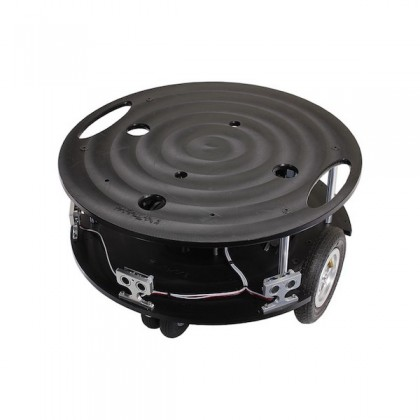
\includegraphics[width=.7\textwidth]{arlo real}
	
	\caption{Mobile robot Parallax Arlo \cite{arloreal}}
	\label{arlore}
\end{figure}


Equally to the Carolo-Cup regulations the lane width is defined by double robot width and therefore 900 mm. 

The robot is equipped with the following sensors:

\begin{itemize}
	\item Lidar
	\item Wheel encoder
	\item IMU
	\item Camera
\end{itemize}

Additional it features a motor driver for differential drive steering.

\section{Software}
Generally the software is developed for ROS-Noetic.\\
The programming language is mostly C++ to allow uniformity in the software stack.\\
Like in the Carolo-Cup the software is not supposed to have any connection to systems outside of the robot.\\

\subsection{Simulation}
Since the environment is simulated the simulator has to have the following features.
\begin{itemize}
	\item Sensor plugins with configurable error and ROS interfaces
	\item Differential drive plugin
	\item Custom models integration
	\item URDF conversion
	\item Not too computationally heavy
\end{itemize}

The simulation is mostly focus on sensor data. That is why sensor plugins with configurable error and a ROS interfaces are needed. Like this the data will be as representative as possible of the real world.\\

In addition to the sensor plugins the simulator needs to provide a plugin for differential drive steering. This is the replacement for the motor controller of the real robot.\\

Custom models is a strict requirement since this thesis focuses on a very specific robot. Furthermore the integration of custom models is necessary to put the robot in different road scenarios.\\

A URDF conversion plugin is very important like this differences between the simulated robot and the tf-tree in ROS can be avoided and the robot will be defined in one file only.\\

To get the best correlation between simulation and real world, the simulator should be able to run close to real time. This will make the simulated sensor data way more reliable and puts the nodes of the navigation\_stack under a realistic load.

\subsection{Navigation}
The navigation is supposed to cover free driving without obstacles, as well as with static obstacles avoidance. It will not cover dynamic obstacles, road sign detection or driving situations like intersections and parking.\\

Development of an entire stack exceeds the content of this thesis, so an open source navigation project will be used which needs to satisfy the following requirements.

\begin{itemize}
	\item Sensor input.
	\item Goal pose input
	\item 2D mobile platform support usage of the conventional drive systems like ackermann and differential
	\item Path planning in respect to the robots kinematic and shape, as well as the environment detected by the sensors.
	\item Path planning and navigation in totally unknown environments
	\item Velocity output as linear and angular velocities
\end{itemize}

\todo{beschreibung}


\chapter{Theoretical Background}
\label{theoretical_background}
This chapter will cover the needed theoretical background about the Gazebo Simulation, the Sensor Plugins, ROS and all of the used ROS packages.

\section{ROS}
ROS (Robot Operating System) is an open Source project developed by the ``Open Source Robotics Foundation''. Like the name suggests it is an entire Operating System for Robots including Hardware abstraction, low-level device control, implementation of commonly used functionality, communication between processes and package management.\\
Furthermore it provides tools and libraries to write, build and run code across multiple computers\cite{rosintro}.\\
\subsection{Packages}
This is the main structure for software in ROS. A package can contain many different Nodes, libraries, service etc.. Furthermore it is the smallest possible Structure that can be build by ROS\cite{rosconcepts}.
\subsection{Nodes}
Nodes are processes that perform computation. Since ROS is very fine granular, a system, that controls an entire robot can contain many nodes that are connected using topics. A package can be written with the use of one of the client libraries roscpp or rospy\cite{rosconcepts}.
\subsection{Plugins}
\subsection{Topics and service}
All of the ROS Nodes are connected with a publisher/subscriber like structure. The topic is basically just a name for a certain message.\\

Not only one node but unlimited many nodes can publish and subscribe to one topic. This generally can be seen like a message bus with not limited connection permissions\cite{rosconcepts}.

Unfortunately the Topic system is not well fitted for request and answers between two nodes, therefore the service structure has been implemented.\\ 
A node might offers a service under a certain node and an other node can call that service. Services can have any in- and output that can be specified in a ``.srv'' file\cite{rosconcepts}.

\subsection{RVIZ}
rviz is a 3D visualization tool offered by default in ROS. It offers functionality to visualize sensor and further geometric data.\\
\subsection{REP}
REP's (short for ROS enhanced proposals) are guidelines made and maintained by the ros community. It is highly advisable to follow the guidelines as much as possible.

Complying to these guidelines allows external people easier comprehension of the structure of the robot and eliminates misunderstandings.

The most important REP's in this project are REP 103 and REP 105.
\subsubsection{REP 103}
	
	"This REP provides a reference for the units and coordinate conventions used within ROS"\cite{REP103}\\  
	
	\textbf{Coordinate Frame}
	\begin{itemize}
		\item \textbf{X-Axis} - Forward
		\item \textbf{Y-Axis} - Left
		\item \textbf{Z-Axis} - Up
	\end{itemize}
	
	\textbf{Units}\\
	Units will always be represented in SI Units and their derived units.\\
	
	\textbf{The order of preference for rotations}
	\begin{enumerate}
		\item Quaternion
		\item Rotation matrix
		\item fixed axis roll, pitch, yaw
		\item Euler angles
	\end{enumerate}
	\cite{REP103}
	
\subsubsection{REP 105}
	"This REP specifies naming conventions and semantic meaning for coordinate frames of mobile platforms used with ROS."\cite{REP105}\\
	
	REP103 Applies for all fixed coordinate frames.
	
	\textbf{Coordinate Frames}
	\begin{itemize}
		\item \textbf{base\_link} is a fixed frame on the robot base. It serves as the reference points for all of hardware mounted on the robot itself like sensors.
		\item \textbf{odom} is a world fixed frame that serves as the reference for the pose of the robot.\\ Since the pose of the robot will drift over time it wont serve as a good long term reference.\\In most cases the odom frame will be computed using localization sensors like wheel odometry, imu's, visual odometry, etc. which leads to a continuous frame.
		\item \textbf{map} is a world fixed coordinate frame that serves as the reference for the odometry frame. It is also the base for a map of the environment such as the ones provided by slam algorithms. The frame is time discrete since it is mostly computed by localization algorithms.
	\end{itemize}
	
	That tree can be extended by an earth frame that would be the reference for the localization of the map in the earth. Which is useful, for long range robot platforms.\cite{REP105}
	
	
	
\subsection{TF}
In most cases robots that are controlled by ros have a so called tf\_tree. This tree is the coordinate frame structure of the robot. In it every sensor and actor has its own coordinate frame.\\
 The structure in most trees of mobile platforms is quite similar which is caused by the REP105 (ROS Enhanced Proposals) this contains a definition of recommended names for the robot frames and their order in the tree. But it should be noted that not every frame that is defined in the norm has to be in every tree. The basic structure mostly starts at a so called fixed frame. This Frame will be the not changing frame in the environment. At moving robots this is often earth, map or odom, while in stationary robots this can even be base\_link.\\
 

The tree is normally build up like in the following image. 

TF2 is the successor of TF and is a very powerful tool in the ROS environment. With it it is possible to transform sensor\_msgs and geometry\_msgs from one frame in another. Furthermore it offers the possibility to transform old data into the present or at any other point in the past.

\subsubsection{URDF and xacro}
The robot hardware description consists of one or more URDF(Unified Robot Description Format) based xml file. Its purpose is to define the shape and geometric of every part of the robot. 

\subsubsection{robot\_state\_publisher}
	This package uses the robot hardware description and builds up the tf\_tree using static\_transform\_publishers.

\section{Gazebo}


\subsection{Plugins}
Gazebo offers a wide selection of pre made plugins that can be incorporated into a simulated robot by attaching the plugin to the right tf\_frame and configuring its parameters.

\subsection{Models}


\section{navigation stack}
\subsection{move\_base}
\subsection{global\_planner}
\subsubsection{base\_global\_planner}
This is the default global planner of move\_base .
\subsection{local\_planner}
\subsubsection{teb\_local\_planner}

\subsubsection{dwa\_local\_planner}
\subsection{costmap}
A costmap is a grid stile map, whose purpose is to store information about obstacles in the surrounding of the robot.\\
There are two different costmaps, the global costmap and the local costmap.
The global costmap is by the global planner to find a collision free path. Whereas the local costmap is used by the local planner for local planning.\cite{navsetup}\\
\begin{figure}[H]
	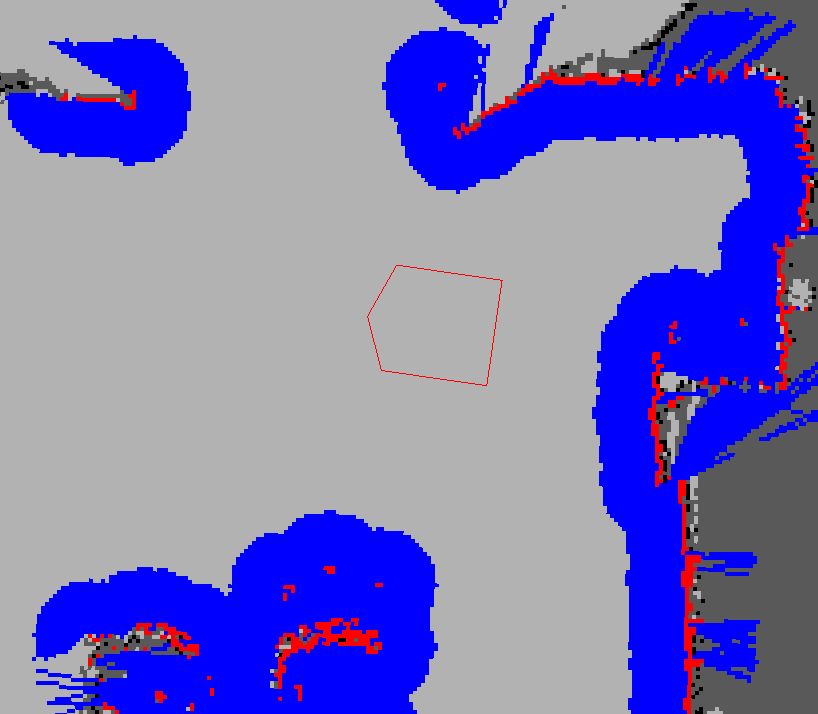
\includegraphics[width=\textwidth]{Pictures/costmap_rviz}
	\caption{costmap with obstacles and inflation \cite{costmap}}
	\label{costmap}
\end{figure}


\subsubsection{Cost Values}
The values in a costmap can be in the range [0-255], but the underlying structure categorizes them in the following 3 sections:
\begin{itemize}
	\item lethal obstacle
	\item free space
	\item no information
\end{itemize}

\subsection{marking and clearing}
Obstacles in the costmap can not only be marked, but also cleared by the subscribed data source. For each data source a configuration regarding the clearing and marking permissions is necessary. For clearing the costmap uses a raytracing algorithm, which allows the costmap to handle moving obstacles\cite{costmap}.
\subsubsection{Inflation}
Inflation is a process where a occupied cell is inflated by over the distance decreasing cost values for a configurable radius, as pictured in Figure \ref{costmap}.\\
This process is used by the default plugin inflation\_layer with the cost distribution pictured in Figure \ref{costdistribution}\cite{costmap}.

\begin{figure}[H]
	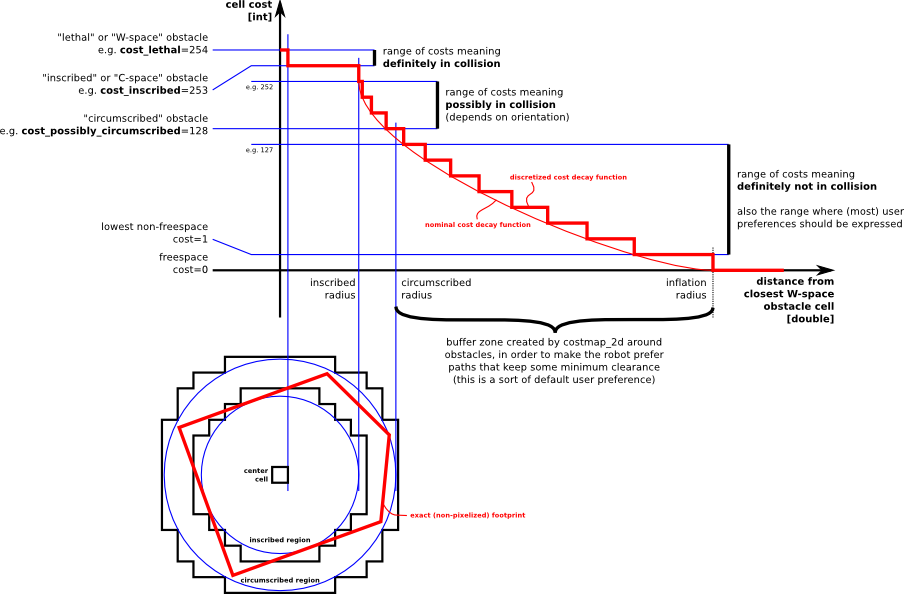
\includegraphics[width=\linewidth]{Pictures/costmapinflation}
	\caption{cost distribution and classification \cite{costmap}}
	\label{costdistribution}
\end{figure}

The usage of inflation has two reasons. First it is used to close gaps between two measured obstacles and therefore usefull, if the sensor resolution is relatively corse.\\
The second reason is to prevent the planner from getting too close to obstacles. Therefore the inflation radius is typically set to slightly more than the radius of the robot\cite{costmap}.

\subsubsection{layer}
The costmap uses a layer structure of plugins that can handle different tasks. The costmap then combines the data from each layer, to produce the final costmap.\\

By default the costmap\_2d package offers the following 3 layers:
\begin{itemize}
	\item \textbf{static map layer} is a layer that converts a prerecorded map into obstacles.
	\item  \textbf{obstacle layer} is a plugin that handles input from sensor sources. The plugin marks and raytraces obstacles in 2D. It can handle LaserScans PointCloud and PointCloud2.
	\item \textbf{inflation layer} handles the inflation of lethal obstacles in the costmap.
\end{itemize}

Furthermore the plugins Social ``Costmap Layer'' and ``Range Sensor Layer'' are offered.

Using the pluginlib interface and the costmap libraries one can develop custom layers for the costmap to achieve special behaviour of the robot.



\section{cartographer}
Cartographer is a Lidar based SLAM developed by Google. In contrast to gmapping it is based on loop closure to ensure real time mapping even in relatively big environments.\\
Submaps are considered for loop closure, if they are close to each other. A scan matcher tries to find constraints between the submaps and the current scan. When searching for loop closure constraints at a certain rate one can achieve basically instantaneous optimization of the map just by the fact that the current scan is similar to one of the underlying submaps\cite{cartographer}.\\

\section{Carolo-Cup}
The carolo cup is an event hosted by University Braunschweig and is an event in which the teams of many different universities can compete against each other and present their work and progress in the field of autonomous driving.

There are two different levels of difficulty the carolo basic cup and the carolo master cup.















%\chapter{Hardware and Software}
\label{hardwareandsoftware}
This chapter will cover the Hardware and Software that was used to set-up, conduct and analyse the tests described in this thesis. 











\chapter{Experimental}
\label{experimental}

In this chapter the setup and qualification process of the the optical and mechanical system is explained.  







\section{The Artificial Eye}
The test setup, which will be described in the following section, was the first physical assembly of the Artificial Eye. It was built after the design, which Chanal described in his report and was the base for the development process described in this chapter. This initial test setup is the first of three development steps described in this thesis. It is marked as orange-bordered in figure \ref{ChainTestSetup}.

\begin{figure}[h]
\begin{center}
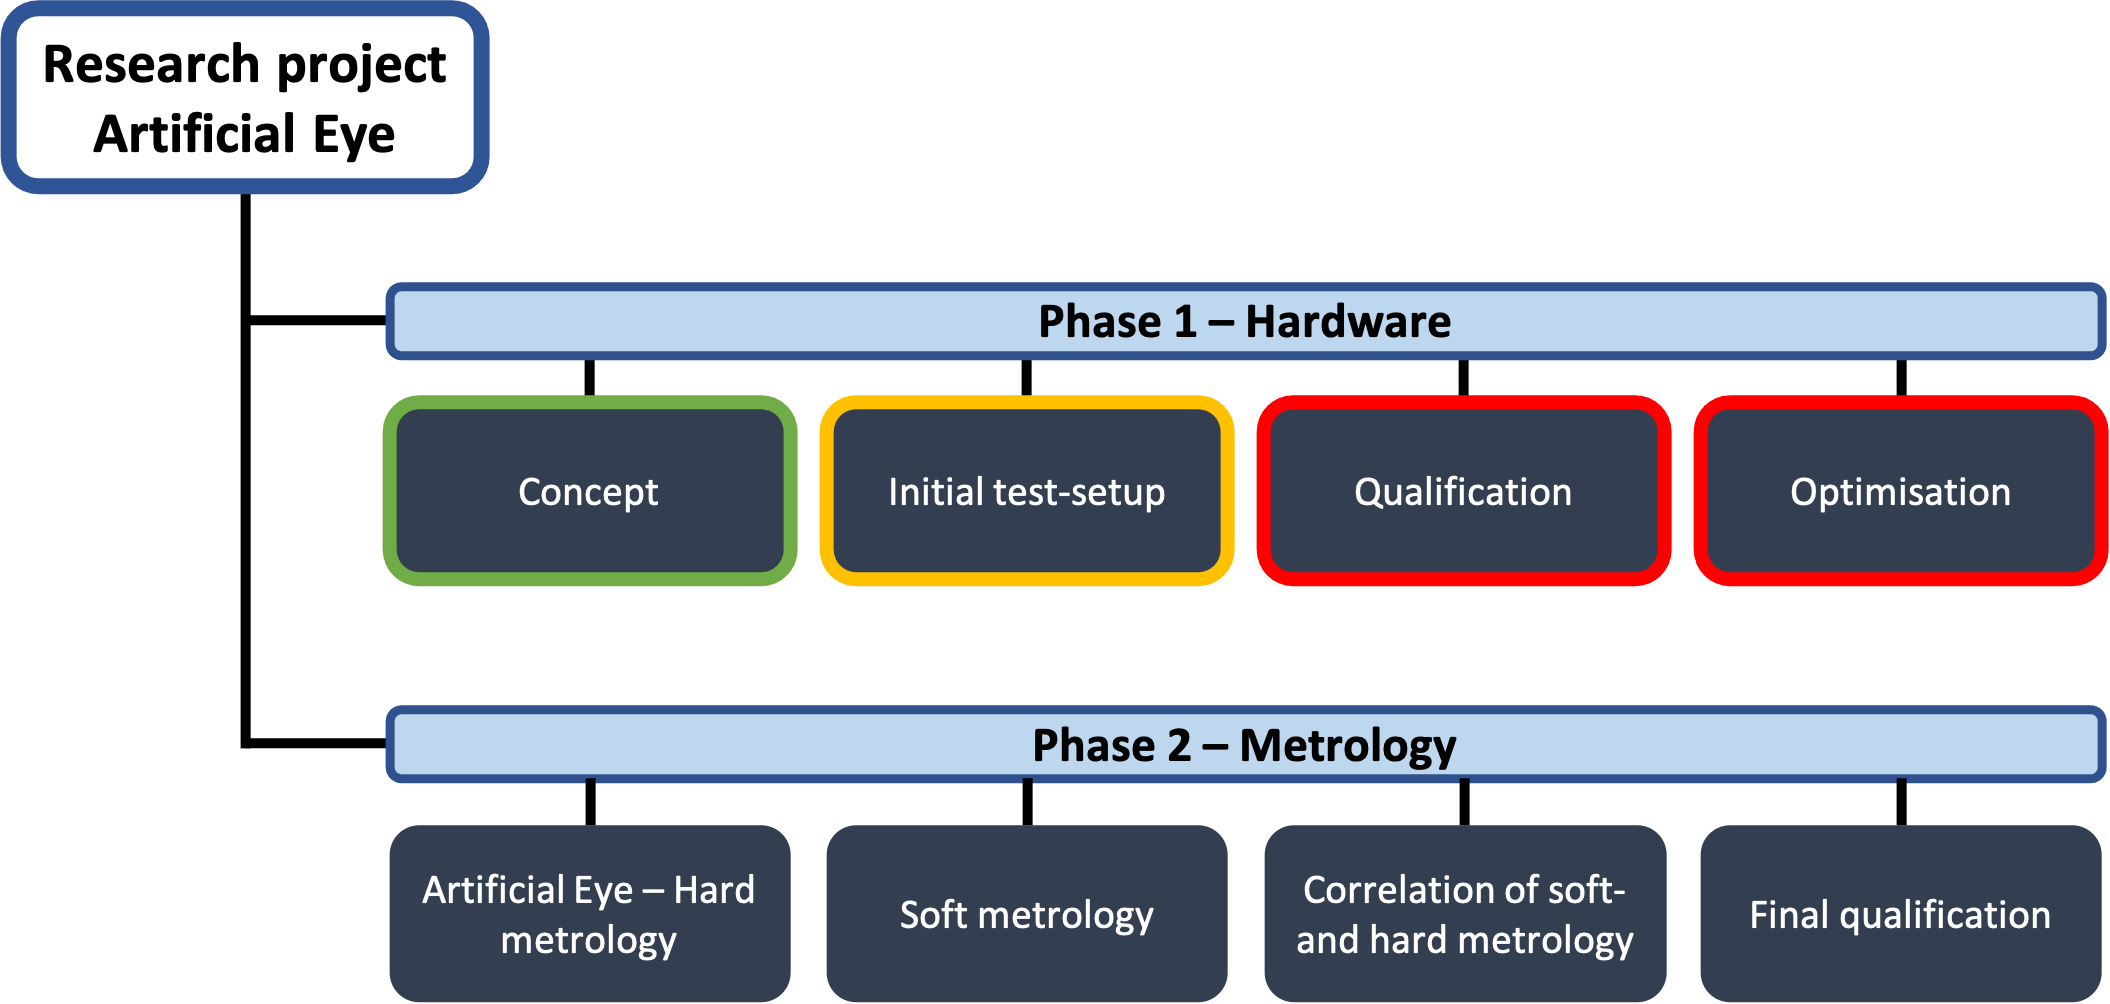
\includegraphics[width=12cm]{Pictures/ChainTestSetup}
\caption[Overview over the development process - Initial test setup]{Overview over the development process - Initial test setup: Green - Completed, Orange - In work, Red - Open}
\label{ChainTestSetup}
\end{center}
\end{figure}


\subsection{Optical system}
The optical system of the Artificial Eye is mostly built to represent the setup of the human eye. Similar to the human eye, the light enters the Artificial Eye through a lens, which focuses the image of the sample on to the light sensors. This lens is a machine vision lens produced by Tamron (see Appendix \ref{AppLoC}) and has a fixed focal length of 75mm and an entry pupil size of 25.5mm. As the human eye, the Artificial Eye has different sensors for colour and light intensity. In the Artificial Eye, these sensors are represented by a system of four digital CMOS cameras with a resolution of 2448 by 2048 pixels and a global shutter. The selected cameras are from the the 5 mega pixel Phoenix series from the manufacturer "Lucid Cameras" (see Appendix \ref{AppLoC}). All four cameras are similar in their sensor and electronics, but differ in the filter pattern which is applied to the physical pixels. On one of the four cameras a standard Bayer-pattern is applied to create a coloured image in software. The three other cameras also have a pattern of filters applied to their physical pixels. But instead of a colour filter this pattern selects different polarisation states of the incoming light. The filter pattern is shown in figure \ref{PHX050S} and filters the incoming light for linear polarisation with the orientation of 90°, 45°, 135° and 0°. In addition to the camera system, the incoming light is also picked up by a Czerny-Turner spectrometer from the company Thorlabs (see Appendix \ref{AppLoC}) to be used as a reference for the camera system.\\
As shown in the digram on the left side of figure \ref{AE_Setup}, the light has to pass through a quarter wave-plate after the lens. The wave-plate will turn right hand polarised light into a 45° linear polarised light and left hand circular polarised light into 135° linear polarised light. Linear polarised light with an orientation of 0° or 90° relative to the fast axis of the wave-plate will not be affected. Next, the light beam is passed through a system of non polarising beamsplitters with a transmission rate of 50/50. The beamsplitter equally distribute the light to the three polarised cameras and to the non-polarising camera as well as the spectrometer. The information of the polarisation of the light can later be used to calculate the surface roughness as well as the material thickness of transparent materials. It is important to note, that similar to an interferometer, a whole section of the sample can be measured at once. This saves time on the one hand, but on the other hand lowers the probability to miss important features of the surface.

\begin{figure}
\begin{center}
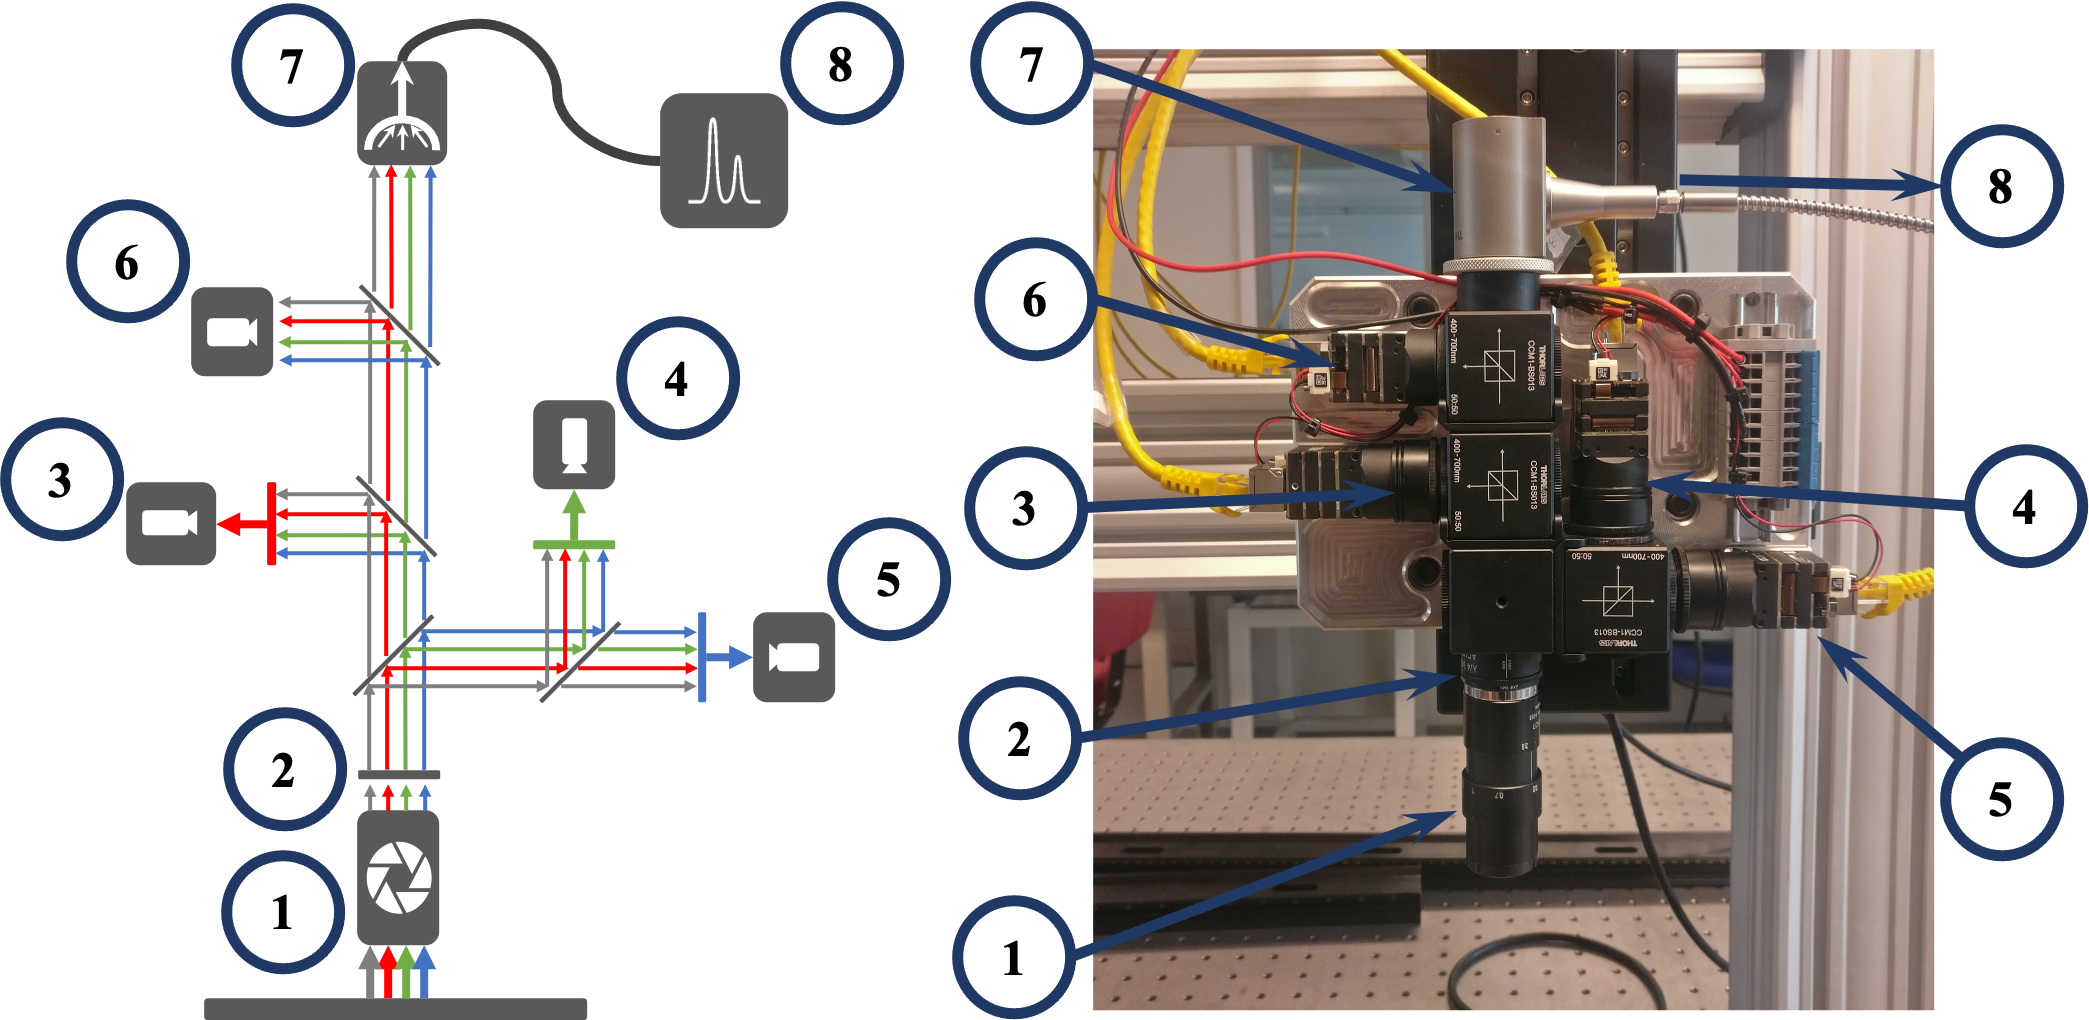
\includegraphics[width=12cm]{Pictures/AE_Setup}
\caption[Schema of the Artificial Eye]{Schema of the Artificial Eye: 1 - Machine vision lens, 2 - Quarter wave plate, 3 - Red filtered camera, 4 - Green filtered camera, 5 - Blue filtered camera, 6 - RGB camera, 7 - Fibre coupler, 8 - Spectrometer}
\label{AE_Setup}
\end{center}
\end{figure}

\begin{figure}
\begin{center}
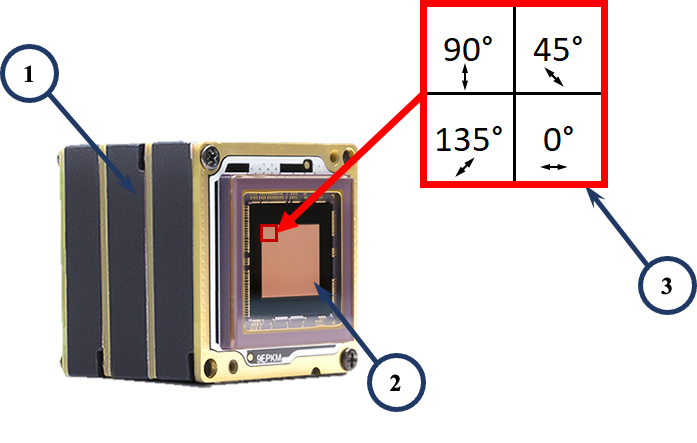
\includegraphics[width=12cm]{Pictures/LucidPHX505s}
\caption[Picture of the Lucid PHX050S Polarised Camera]{Picture of the Lucid PHX050S Polarised Camera\cite{Labs}: 1 - PHX050S Camera, 2 - CMOS Sensor, 3 - Detail of the polarisation pixel pattern}
\label{PHX050S}
\end{center}
\end{figure}

In order to represent the cones of the human eye, which are responsible for the colour vision in the human eye and only see a very small portion of the electromagnetic spectrum, the light is filtered similarly before being picked up by the polarised cameras. This is done with bandpass filters with a Bandwidth (FWHM) off 10 nm, with a CWL of 420 nm for the blue, 530 nm for the green and 620 nm for the red spectrum. This part of the Artificial Eye is responsible for colour-metric measurements, similar to a spectrophotometer. 


\subsection{Mechanical system}
The mechanical system built for the Artificial Eye consists of three linear travel stages arranged as a 3-axis cartesian motion system. The three axes are arranged in a way that the measurement setup is only moving in one axis, in Z. This has the advantage, that the heavy camera system only needs to move when it is necessary to adjust the focus. The sample will then be placed on the two remaining axes which are arranged as "X-Y table". Both, X-Y table and Z axis are mounted as shown in figure \ref{MotionSystem} on top of an optical table (to read more about optical tables see Appendix \ref{AppendixAdditionalTopics}).\\
It was necessary to calibrate the motion system to ensure that the X and Y axis are mounted in 90° angle to each other. Further, the Z axis with the measurement setup needed to be mounted perpendicular to the X-Y Table. This calibration was done with the help of the camera system of the Artificial Eye.\\
First the Z axis was calibrated. This was done by focusing the camera system on a specific point on the optical table. As a next step the camera system was moved towards the optical table and the focus of the lens was adjusted until the camera image was sharp again. As soon as the Z axis was perpendicular to the surface of the optical table, the point of interest remained in the center of the Field of View (FOV) during movements in Z.\\
For X and Y, the system was focused onto one edge of the X-Y table. One of the axes was then moved by 20 mm. After the movement, the position of the edge was compared to its initial position. If the table only moved along the axis of intended movement, the rotation of the moved axis (relative to the rest of the system) could be declared as good. Was the edge slightly wandering off into one direction perpendicular to the direction of movement, the moved axis was slightly rotated around the Z axis and needed to be corrected. This process was repeated multiple times for both, X and Y axis in order to complete the calibration.

\begin{figure}
\begin{center}
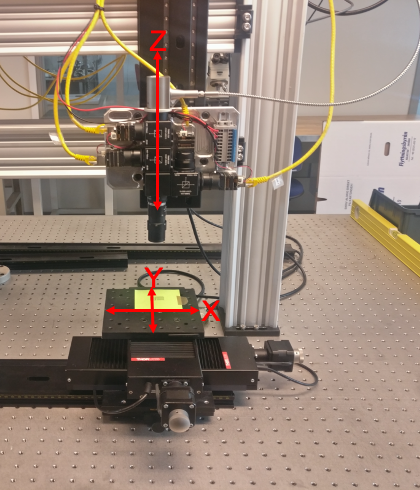
\includegraphics[width=12cm]{Pictures/MotionSystem}
\caption[Picture of the motion system of the Artificial Eye]{Picture of the motion system of the Artificial Eye}
\label{MotionSystem}
\end{center}
\end{figure}


\subsection{Electrical system}
In order to operate the Artificial Eye and acquire data from the camera system and the spectrometer a power and data connection needed to be provided to the setup. To avoid timing problems with the camera system and run the cameras at a cooler temperature, the decision was made to not to use the POE (Power over Ethernet) capability of the cameras. The camera system was powered with an external 24V Power Supply.\\ 
Figure \ref{ElectricalSetup} shows the overview of the electronic circuit:

\begin{enumerate}
	\item \textbf{Schuko plug type F:} The Schuko plug is connected to an 230 VAC power outlet to power the circuit.
	\item \textbf{Phoenix Contact Mini PS 100:}The power supply converts 230 VAC to 24 VDC. It has a maximum power output of 48 W. It can operate in a temperature range from -25 °C to 60 °C.\cite{RSComponents}
	\item \textbf{Cat. 5E Ethernet cable:} The Cat. 5E transfers the data from the camera system and the USB Hub to the Ethernet switch. Both ends have a male RJ45 connector.
	\item \textbf{Camera System:} The camera system can be powered with both, power over Ethernet (POE) or 12 VDC to 24 VDC external power. To avoid interferences in the Ethernet cable when using POE the camera system was powered with an external source of 24 VDC. As data connection a 100 MBps (Million Bits per second) ethernet connection was used.
	\item \textbf{Thorlabs CCS 100/M Spectrometer:} The CCS100/M is the metric version of Thorlabs compact CCD spectrometer series. It uses a rugged Czerny-Turner spectrometer design with no moving parts. The wavelength range of the spectrometer is 350 nm to 700 nm with a spectral accuracy $<$0.5 nm at 435 nm. The spectrometer was connected to the USB Hub with a USB-A to Mini USB-B Cable. The input light was coupled into a optical fibre with a reflective coupler.\cite{ThorlabsCCS}
	\item \textbf{Thorlabs reflective coupler:} The RC12FC-P01 is a reflective collimator and coupler by the company Thorlabs. It can be used for a wavelength range from 450 nm to 2 $\mu$m and has a input/output opening of 12 mm.\cite{ThorlabsCoupler}
	\item \textbf{DIGI 14 Port USB Hub:} The 14 port USB Hub manufactured by the company DIGI (see Appendix \ref{AppLoC}) offers 14 USB2.0 or 3.1 ports for extension over Ethernet. It can be mounted in a standard 19" server rack. 
	\item \textbf{MikroTik 24 Port Ethernet Switch:} The MikroTik (see Appendix \ref{AppLoC}) 24 Port Ethernet switch is the central point of the Ethernet network. It connects all devices to the host computer and manages their communication.
\end{enumerate}

\begin{figure}
\begin{center}
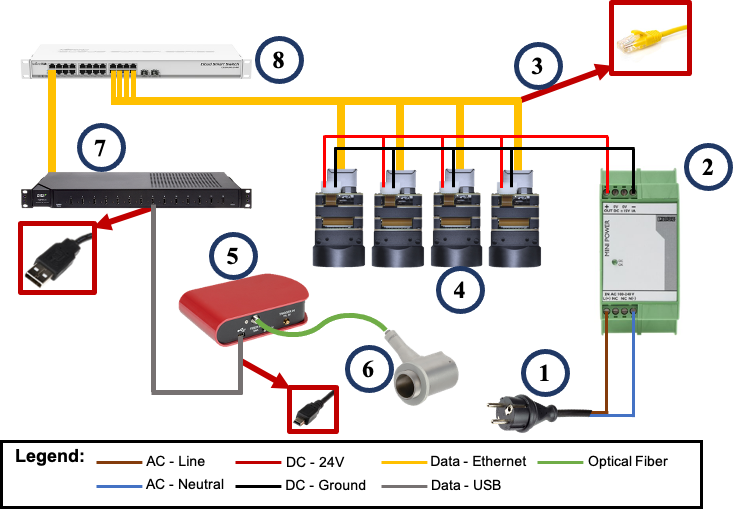
\includegraphics[width=12cm]{Pictures/Electrical Setup}
\caption[Electronic Circuit of the Artificial Eye:]{Electronic Circuit of the Artificial Eye: 1 - Schuko plug type F\cite{MuellerPlastik}, 2 - Phoenix Contact Mini PS 100\cite{RSComponents}, 3 - Cat5e Ethernet Cable\cite{ComputerCableStore}, 4 - Camera system\cite{Labs}, 5 - Thorlabs CCS 100/M Spectrometer\cite{ThorlabsCCS}, 6 - Thorlabs reflective coupler\cite{ThorlabsCoupler}, 7 -  DIGI 14 Port USB Hub\cite{DIGI}, 8 - MikroTik 24 Port Ethernet Switch\cite{MikroTik}}
\label{ElectricalSetup}
\end{center}
\end{figure}

\subsection{Software}
The acquisition, processing and evaluation of the data collected by the camera system and the spectrometer was done with a program created in LabVIEW (see Appendix \ref{appendixSoureCode}). This could be compared to the function of the human brain, which also acquires, processes and evaluates the pictures collected by the eyes. In order to have a clearly structured, maintainable as well as expandable software, the program was split into multiple subprograms. The so called "Sub-VI's" all have their own specific task such as configuring the camera system, processing the images or saving the resulting data.\\

\begin{figure}
\begin{center}
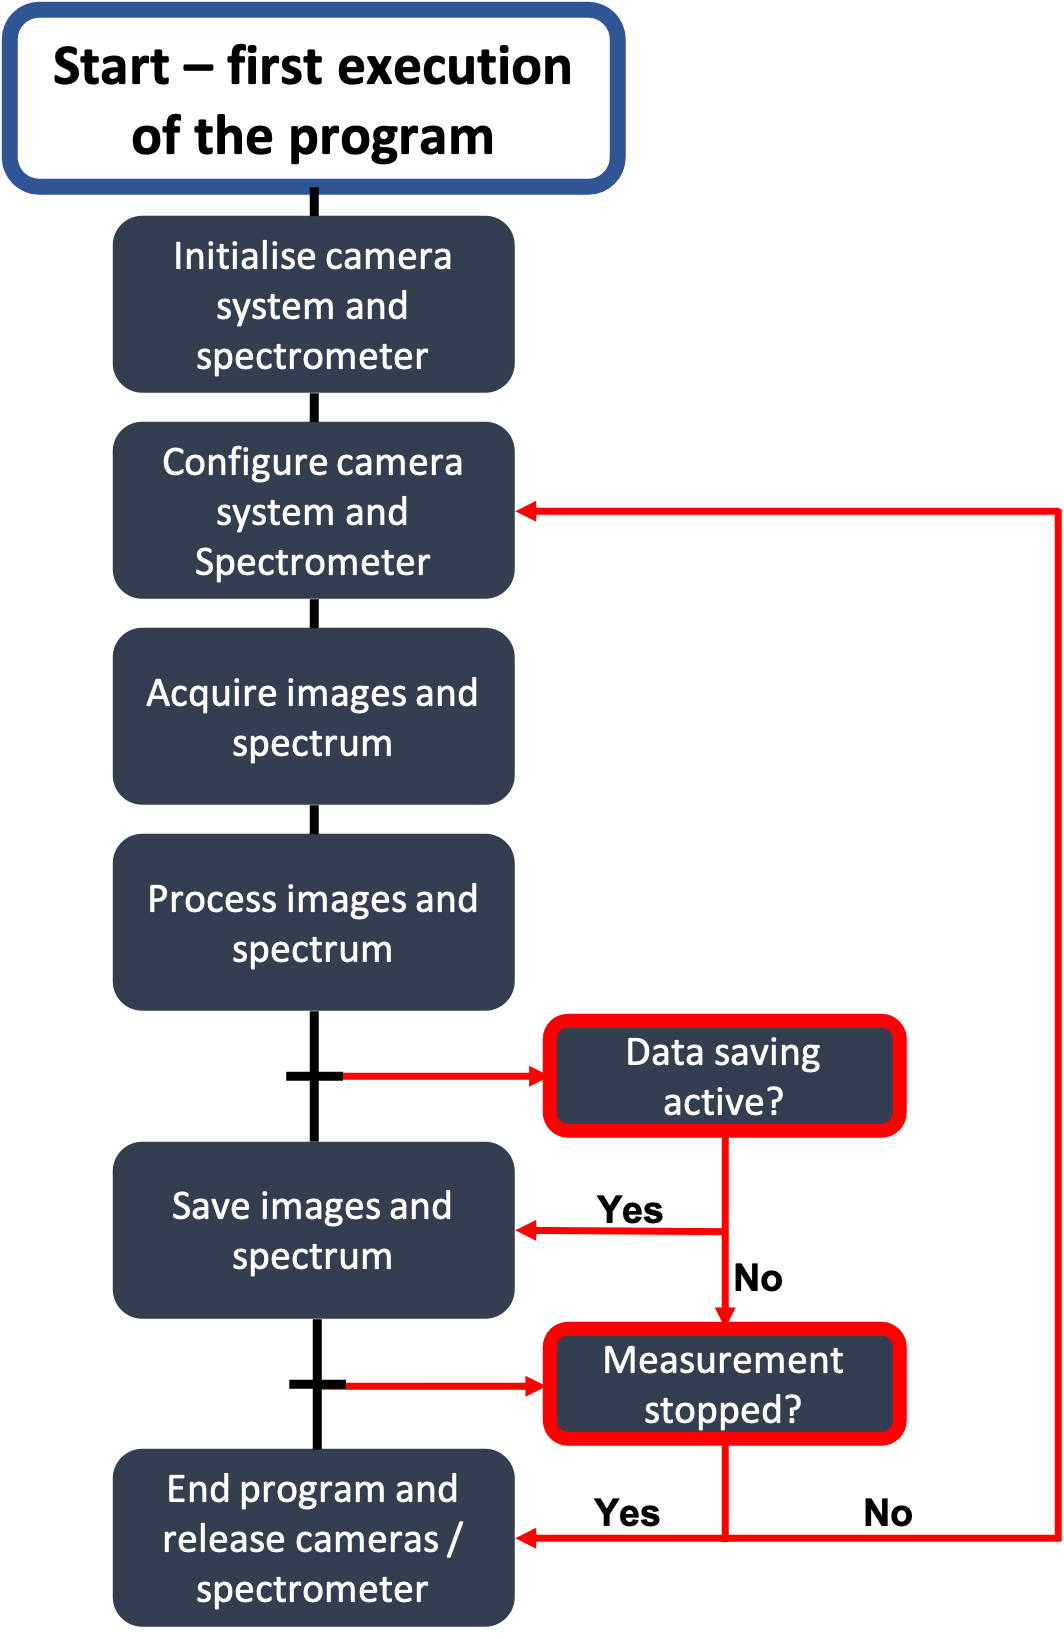
\includegraphics[width=12cm]{Pictures/MainVI}
\caption[Flowchart of the LabVIEW program]{Flowchart of the Labview program}
\label{MainVI}
\end{center}
\end{figure}

A flowchart of the Program is shown in figure \ref{MainVI}:

\begin{enumerate}

	\item \textbf{CamInit.vi and SpecInit.vi:} The subprograms "CamInit" and "SpecInit.vi" are responsible to initialise the connection to the camera system and the spectrometer. They house all functions needed to establish the serial connection via Ethernet to the five devices. These functions are only executed once, at the start of the program.
	\item \textbf{CamConf.vi:} This subprograms configure the acquisition parameters for the camera system. It is responsible to send the acquisition parameters such as exposure time, analogue gain, field of view to the devices. To be able to adjust these parameter while the program is running, this subprogram has to be executed every acquisition cycle.
	\item \textbf{CamAcqu.vi and SpecAcqu.vi:} The acquisition of the images happens in the subprograms "CamAcqu.vi" and "SpecAcqu.vi". In order to lower the traffic on the Ethernet connection, the acquisition of the data is handled separately for each of the cameras and the spectrometer. This means that the data acquisition of camera 1 has to be finished before camera 2 is allowed to send data. 
	\item \textbf{Processing.vi:} "Processing.vi" is the core function of the the Artificial Eye software. It takes the raw images as inputs and outputs the processed images. This subprogram corrects mirrored and flipped images caused by the beamsplitters and mounting of the cameras.
	\item \textbf{ImSave.vi:} As last step the acquired images as well as the spectrum are saved to the hard drive of the computer. This is done to be able to evaluate the data in post processing with programs like MATLAB. The images are saved as complete 2048x2048 16 bit unsigned integer binary file. Further, each of the images is split and saved as a smaller partial image with a resolution of 1024x1024. These images only contain one polarisation or in case of the RGB camera one of the four intensities produced by the bayer pattern. This is done by splitting the image into four before saving. The spectrometer data will be saved as a .csv (coma-separated values) file. In order to not fill up the hard drive with useless data, saving can be activated or deactivated. When active the LabVIEW function will create a new folder, marked with date and time, for each new acquisition cycle. Data saving is turned off by default.
	\item \textbf{Main.vi:} The program "Main.vi" is responsible to control all subprograms. This program will be used by the operator. It will run the device configuration, data acquisition, data processing and saving in an infinite loop, until interrupted by the operator.
	\item \textbf{Visualisation:} The front panel of the program Main.vi represents the GUI which will be used by the operator of the system. It will show a live view of the camera and spectrometer data and enables the operator to interact with the system. It offers the controls to change the gain and exposure time for each camera and set the integration time of the spectrometer. Further it enables the user to start and stop the program as well as to enable and disable the saving feature. The latest version of the Main.vi front panel is shown in figure \ref{Frontpanel}.
\end{enumerate}

\begin{figure}
\begin{center}
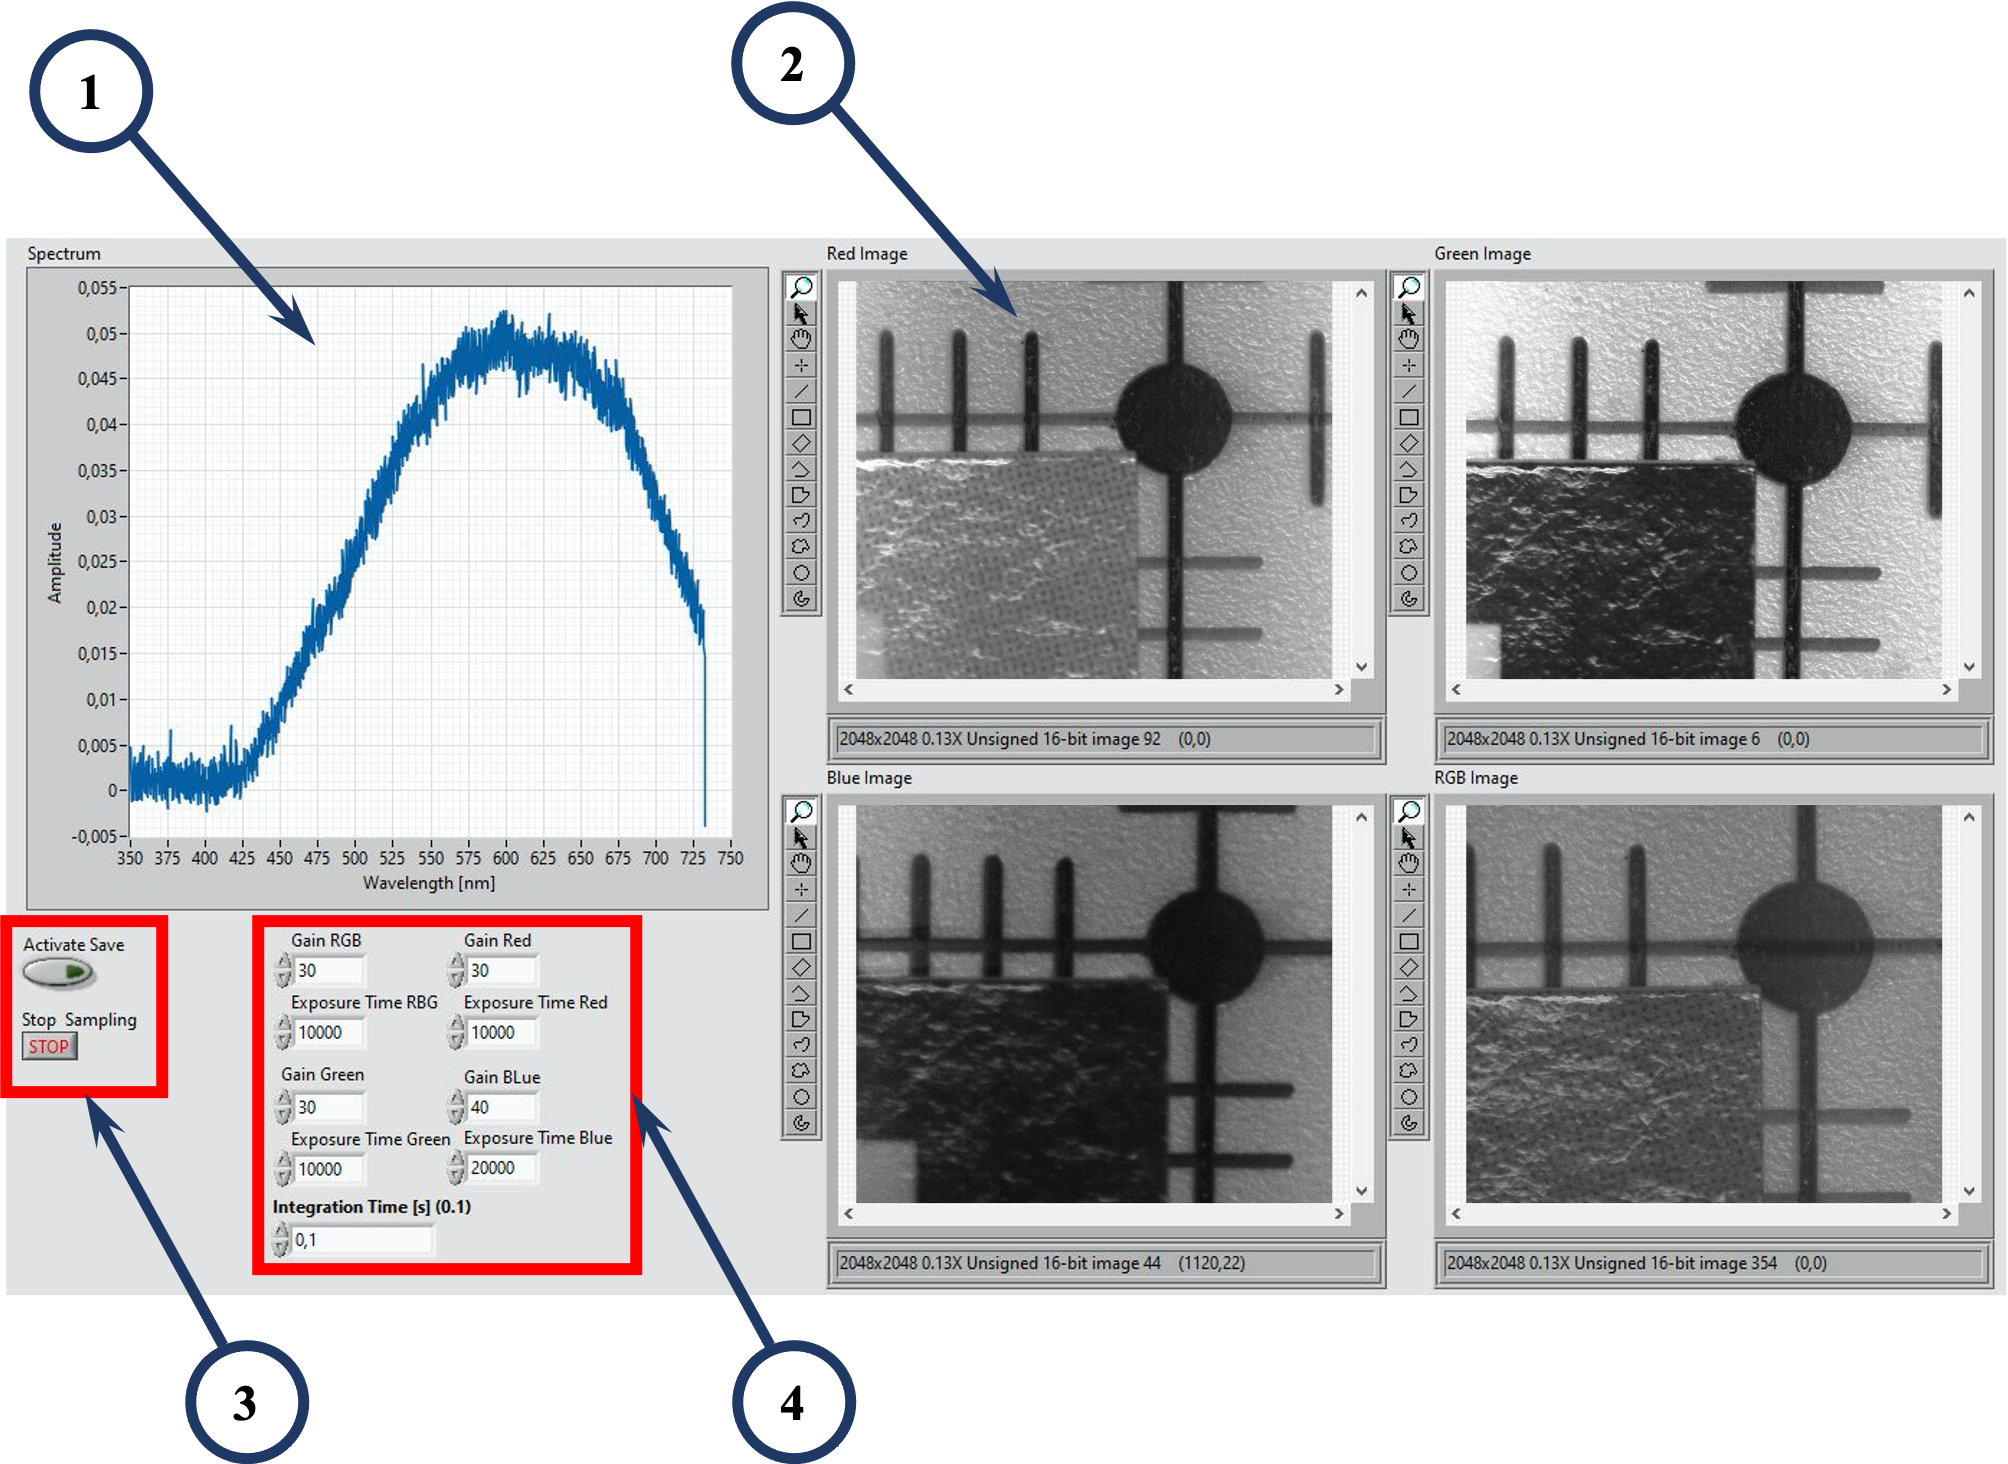
\includegraphics[width=12cm]{Pictures/Frontpanel}
\caption[Image of the LabVIEW front panel for the control of the Artificial Eye]{Image of the LabVIEW front panel for the control of the Artificial Eye: 1 - Graph with the captured spectrum, 2 - Camera images, 3 - Controls for saving and stop, 4 - Controls for device parameters}
\label{Frontpanel}
\end{center}
\end{figure}




\section{Transmission test} 
The testing of the initial setup is part of the qualification and therefore the second step in the first phase of the development of the Artificial Eye. It is shown as orange-bordered in figure \ref{ChainQuali}.

\begin{figure}[h]
\begin{center}
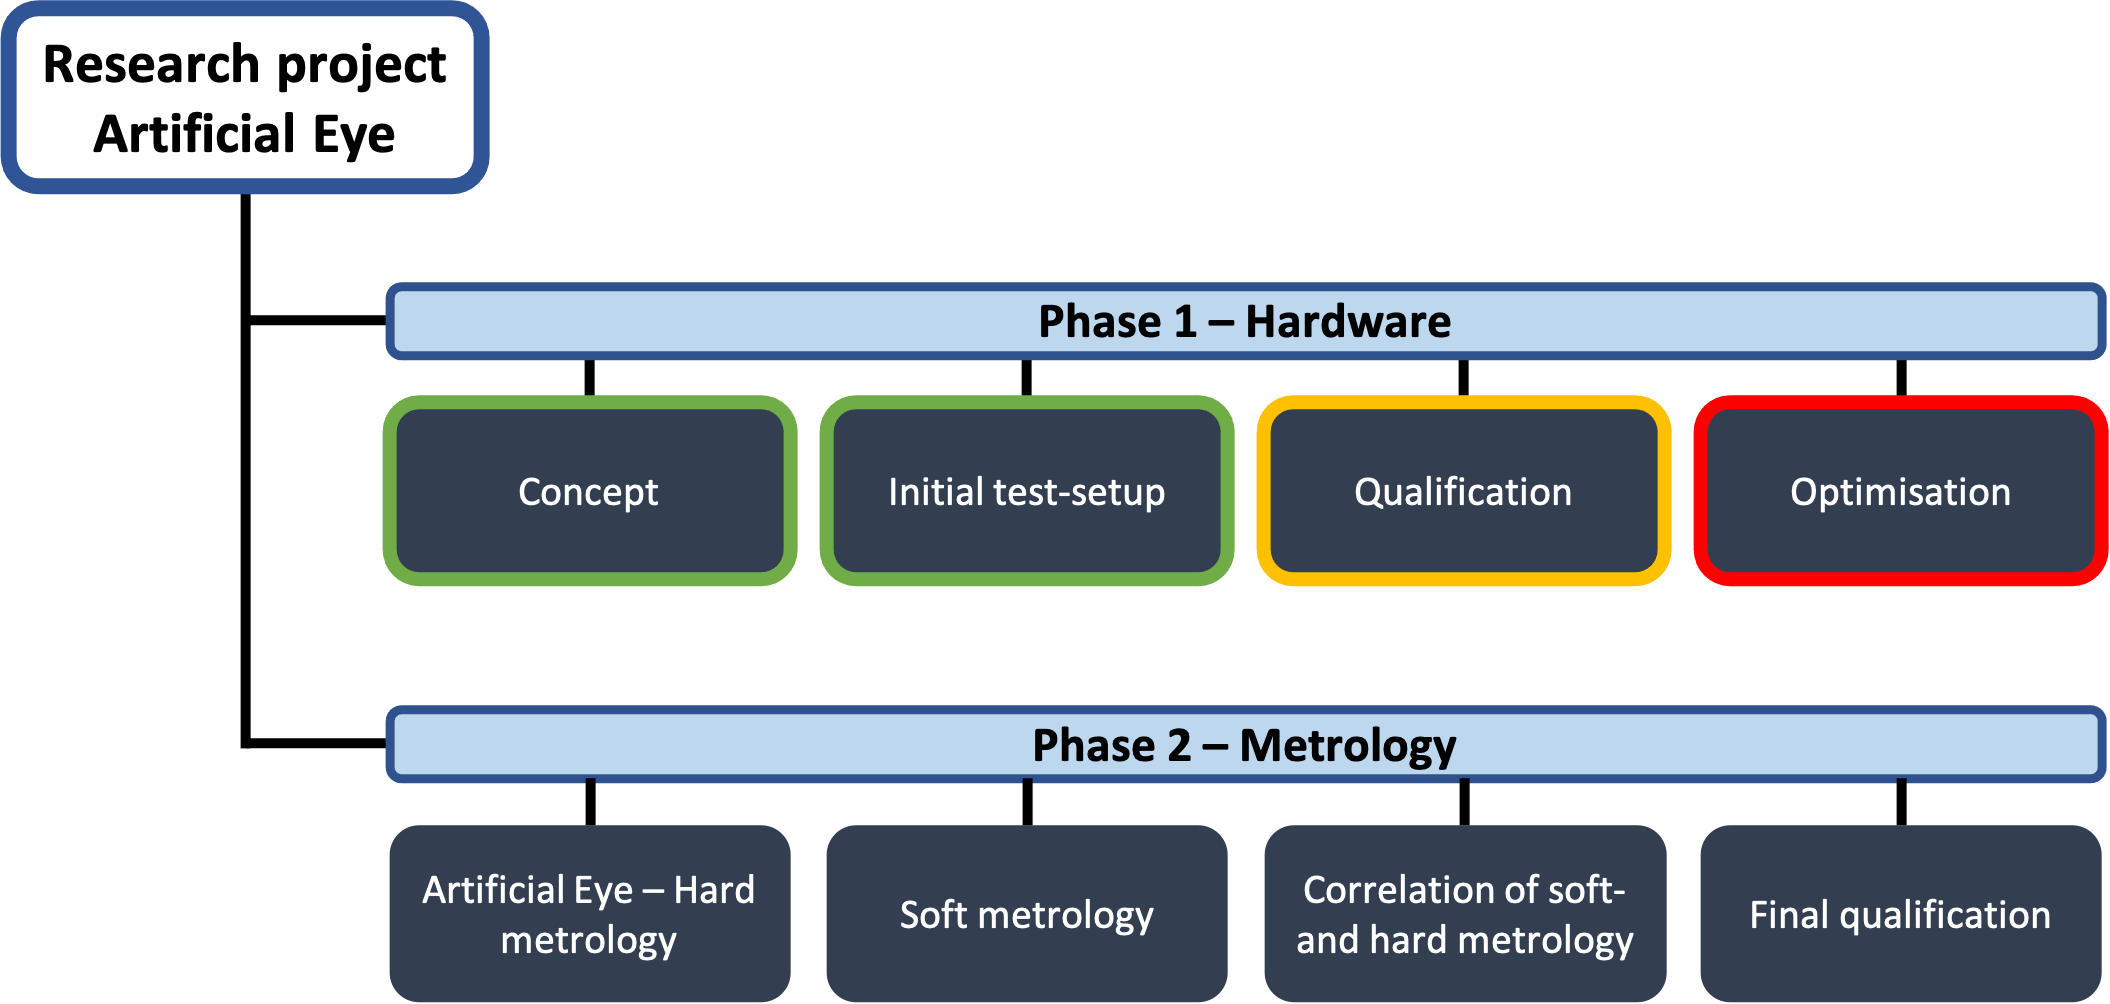
\includegraphics[width=12cm]{Pictures/ChianQuali}
\caption[Overview over the development process - Qualification]{Overview over the development process - Qualification: Green - Completed, Orange - In work, Red - Open}
\label{ChainQuali}
\end{center}
\end{figure}

This test was aimed to investigate, if the selected bandwidth of the colour filters and the transmission of the optical system is sufficient. Further the right exposure time and analog gain (amplifier) settings for the camera system need to be configured. In order to focus the camera system, a reference object was needed. During the execution of this testing series, two different types of references were used:
\subsubsection{Fine grid plate}
The reference which was used first, was a matt black rectangle made from acrylic. The acrylic was then laminated with a matt white vinyl in order to create a surface which reflects light well, but does not cause glare or direct reflections. Further, a fine grid structure was laser-etched into the white vinyl. With the acrylic as backgrounds, the grid was visible as a high contrast structure. This was used to focus the camera system and reference the position of its point of view.
\subsubsection{Illumination source}
To illuminate the reference plate, an incandescent light bulb was used. This type of light bulb provides a smooth spectrum, gradually increasing in intensity from 400 nm into the near infrared spectrum. The light intensity of the bulb was measured to be $\sim$18000 lux on the surface of the reference plate. This is roughly the intensity of daylight. The lightbulb was placed at the same hight as the optical system and the light was pointed onto the surface of the test plate at an angle of $\sim$45° in order to avoid direct reflections or glare. The spectrum of the lightbulb is shown in figure \ref{AMOLEDSpectrum}. \\

\begin{figure}
\begin{center}
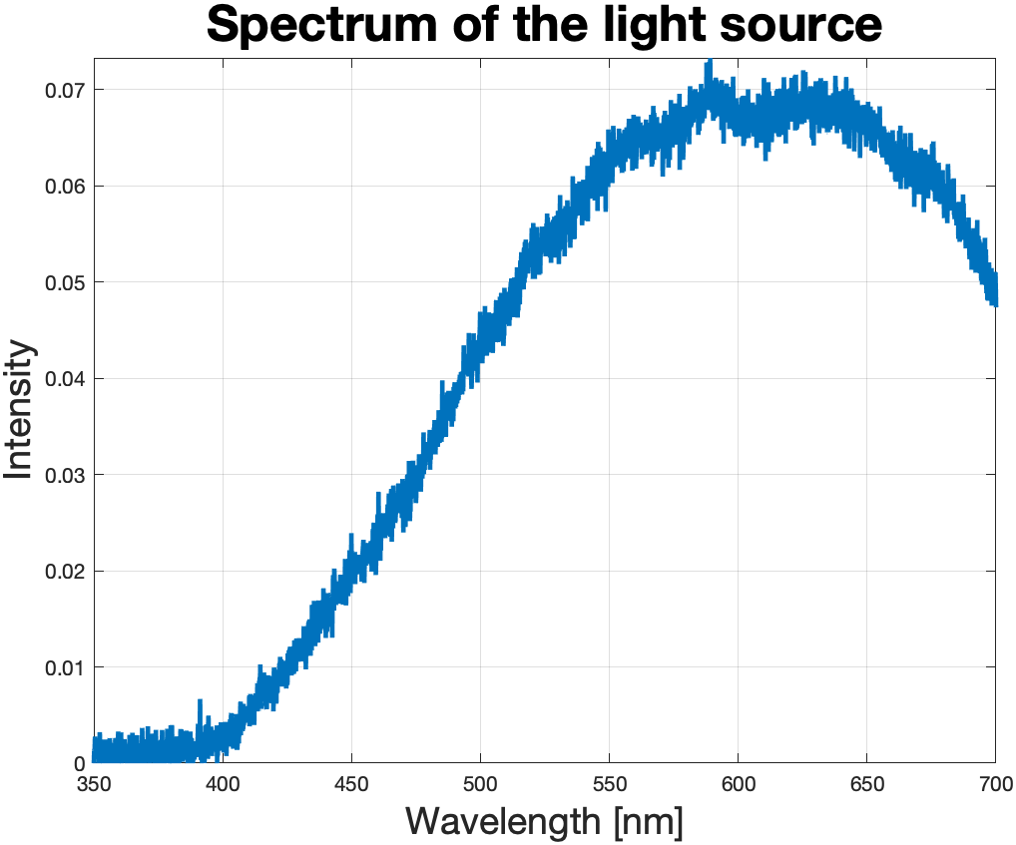
\includegraphics[width=12cm]{Pictures/AMOLEDSpectrum}
\caption[Graph showing the spectrum emitted by the incandescent light bulb]{Graph showing the spectrum emitted by the incandescent light bulb}
\label{AMOLEDSpectrum}
\end{center}
\end{figure}

In order to find a common value for the gain for all cameras in the system, the test was setup to try a variety of different values. The test was executed by setting all four cameras to the same exposure time and analog gain and saving the resulting images for evaluation. As starting values, the highest possible gain (48 dB) and an exposure time of $\frac{1}{1000}$ s was selected. The gain was then lowered in 5 dB steps. To ensure that the intensity of the illumination was consistent for all measurements, the intensity of the incoming light was measured and saved with the spectrometer. To make the data of the RGB camera comparable to the other three cameras in the setup, its was configured to output a greyscale image with a colour precision of 12 bit. This is the default output format for the three monochromatic cameras. In order to have a reference for the point where an image is too dark, a reference image was taken. This was done by adjusting the gain of the RGB camera while evaluating the brightness of the image shown in a live feed of the camera.


\section{Focus test}
The aim of this test was to ensure that all four cameras are sharing the same focal point. This is needed in order to take quick measurements without the need to readjust the focus for each of the cameras in the system. As a reference for the focus and point of view of the system, the fine grid plate was used. To measure the difference in focus and point of view between the cameras, the linear axes were used.\\
The procedure to measure the deviation between the cameras was as follows:
\begin{enumerate}
	\item The reference plate was placed in the center of the X-Y table.
	\item The connection with the camera and the Thorlabs linear axes where established. The linear axes need to be homed (referenced to the zero point of the axis)
	\item One of the cameras was selected as a reference for the remaining cameras. In this case the RGB camera was set as a reference. 
	\item The selected camera was focussed onto the reference plate.
	\item The crosshair in the center of the reference plate was moved into the FOV of the camera using the X-Y table. The inner most reference lines on the plate where aligned with the left and upper edge of the image (see figure \ref{XYZCalibSetup} right).
	\item The position of the X,Y and Z axis were noted down, as reported in the Thorlabs control software (see figure \ref{XYZCalibSetup} left). 
	\item The steps from 4. - 6. were repeated for all cameras in the system.
\end{enumerate}

\begin{figure}
\begin{center}
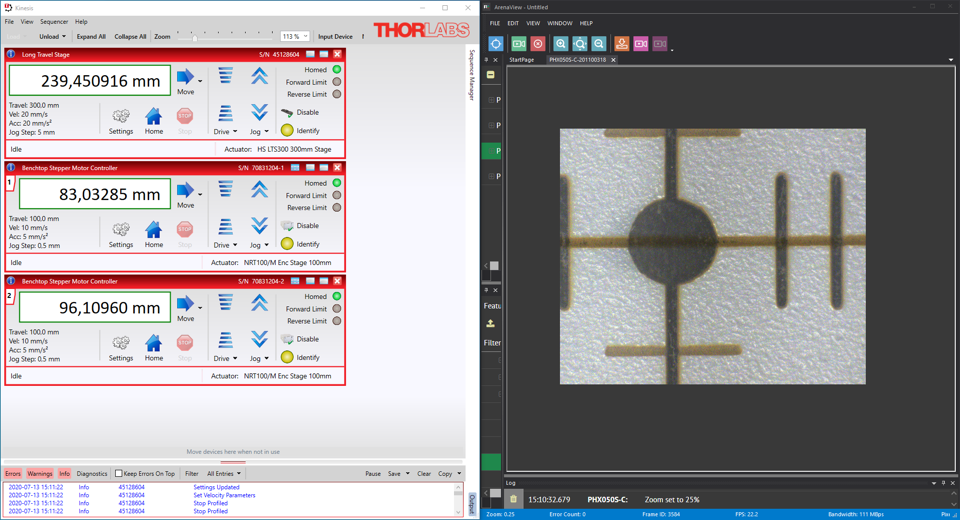
\includegraphics[width=12cm]{Pictures/XYZCalibSetup}
\caption[Picture of the process to calculate the offset of the camera system in X,Y and Z]{Picture of the process to calculate the offset of the camera system in X,Y and Z: Left - Position information of the Thorlabs linear axis system, Right - Live image of the RGB camera}
\label{XYZCalibSetup}
\end{center}
\end{figure}



\section{Resolution test}
As the human eye has a maximum resolution of 200 $\mu$m at a distance of 700 mm, it needed to be ensured, that the Artificial Eye has a similar or higher resolution. The distance of 700 mm has been chosen, because it is often used in the industry to inspect parts. One reason for that is, that 700 mm is roughly the length of an arm. Therefore it is a quick and easy solution to inspect parts at a reproducible distance in a production environment. The testing series to investigate the maximum resolution of the optical system of the Artificial Eye was conducted after the previous two tests were evaluated and therefore the initial setup of the Artificial Eye was already slightly changed. The most remarkable change to note is the different lens used in this revision of the Artificial Eye. In contrast to the old lens, the new lens features an adjustable focal length (zoom). Adjusting the focal length, widens or narrows down the FOV. At 700 mm the maximum FOV is 68x55 mm, the minimum FOV is 17x15 mm. For this reason, the resolution test has to be done for both, the maximum and minimum FOV at a viewing distance of 700mm.\\
Because there was no vertical mounting option to achieve a distance of 700 mm between the lens and the sample, the artificial eye was mounted horizontally onto the optical table. This also caused that the X-Y table could not longer be used, because it is not possible to mount it on its side. The linear axis, which was used as Z axis in the earlier setup, could still be used to adjust the focus of the system remotely.\\
To determine the maximum resolution of the optical system a calibration plate was used. This calibration plate was placed 700 mm in front of the lens of the Artificial Eye. It has a micro pattern of lines machined into its surface. The pattern consists of lines, equally spaced, with a thickness ranging 1 $\mu$m to 600 $\mu$m. Both, the complete test-setup as well as a detail of the calibration plate are shown in figure \ref{ResolutionSetup}.

\begin{figure}
\begin{center}
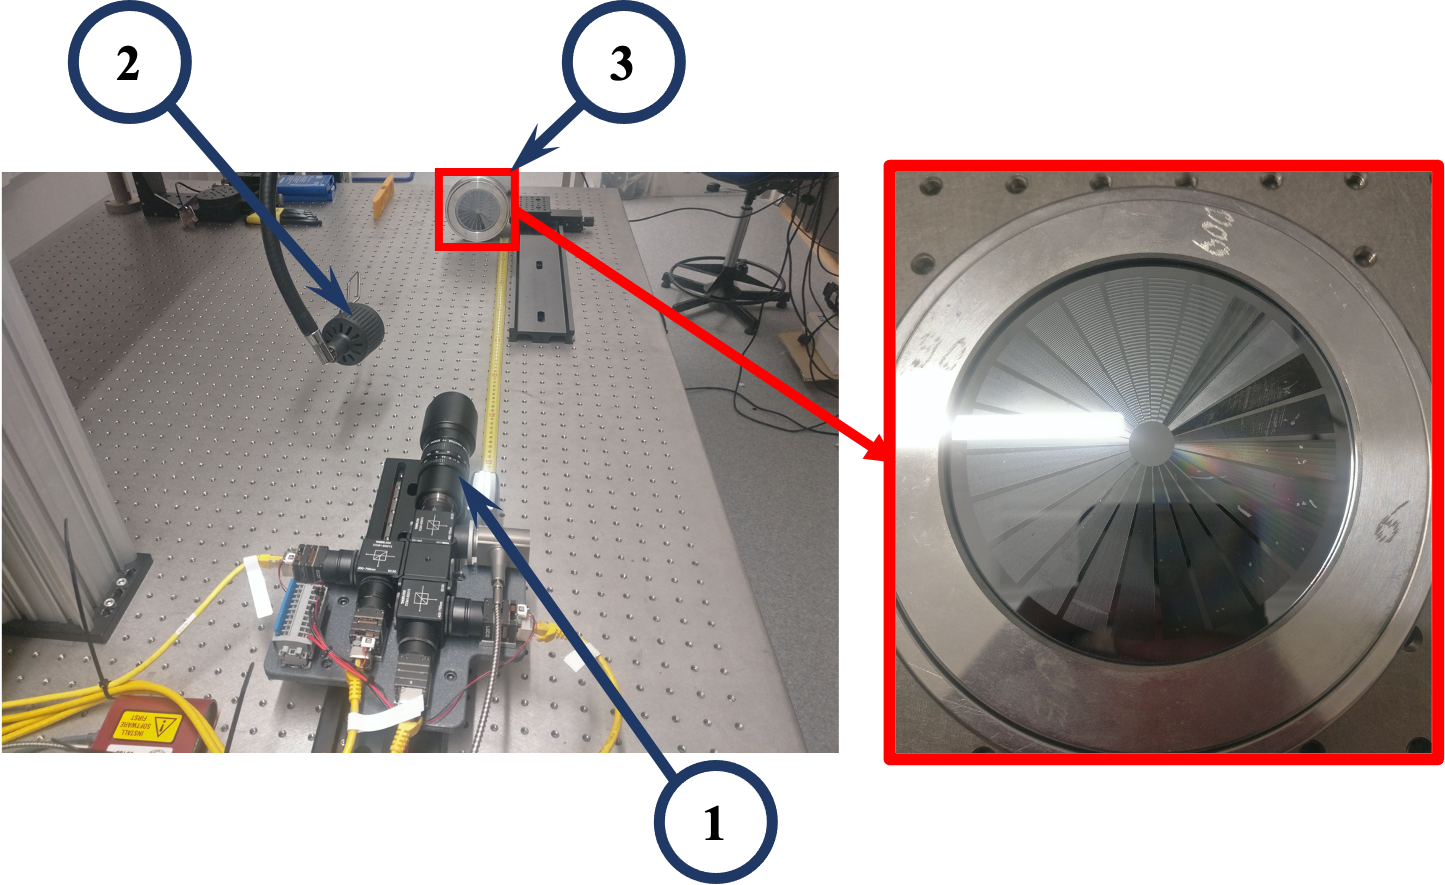
\includegraphics[width=12cm]{Pictures/ResolutionSetup}
\caption[Picture of test-setup for the minimum resolution tests]{Picture of test-setup for the minimum resolution tests}
\label{ResolutionSetup}
\end{center}
\end{figure}







\chapter{Results and Discussion}
\label{resultanddiscussion}


This chapter covers the results and the discussion of all tests formulated in Chapter \ref{configurationandtesting}. In addition potentially needed optimization steps will be highlighted.
\section{Odometry test}

When looking at the odometry published by the differential drive plugin during the test in Figure \ref{wheel odom} it is noticeable, that the measurement has a huge rotational error, which is expected since the wheels always slip slightly when turning a differential drive robot.
\todo{picture including true odometry}
\begin{figure}[H]
	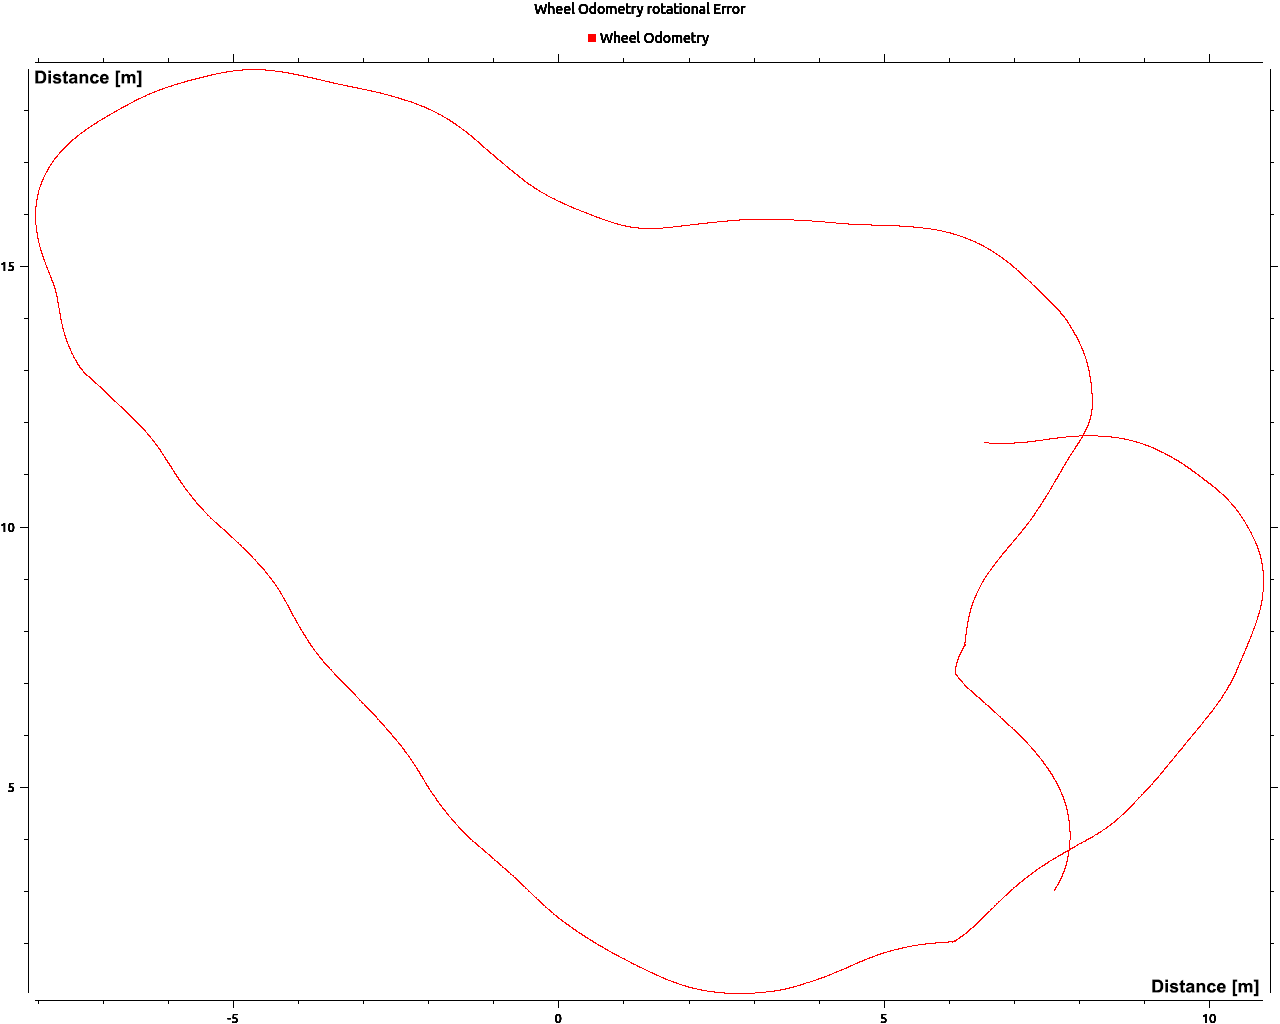
\includegraphics[width=\textwidth]{Pictures/rot error}
	\caption{Odometry Test result}
	\label{wheel odom}

\end{figure}

The quality of the odometry obviously is not sufficient and has to be improved.

\subsection{Optimization}
Since the odometry is found to not being sufficient for the navigation the following optimization approach will be tried and further testing will be performed. The test scenario will be remain the same.

To improve the odometry the ROS package robot\_localization can be used. It provides an extended kalman filter for the fusion of sensor data for odometry.\\

To reduce the rotational error, an IMU (Inertia measurement unit) will be added to the robot configuration. Both, the imu and the wheel encoder will be fused by robot\_localization.

The IMU provides the following data:
\begin{itemize}
	\item orientation
	\item angular velocity
	\item linear acceleration
\end{itemize}

In this usecase the IMU is only supposed to measure data relevant for 2D operation roll, pitch and tranlation in z (axis according to to REP 103) will not be passed to the filter. 

The IMU is used for localization purposes, therefore the linear acceleration data is not interesting, since the accelerations would need to be integrated twice to be used for the pose. This would amplify every little error in the measured acceleration and will decrease the reliability of the odometry with increasing time.\\

Accordingly the only things fused from the imu are the yaw orientation and velocity.\\

Just like the IMU data the integration of the wheel-odometry data has to be discussed which consist only from linear and angular velocities, aswell as a pose derived from the velocities.\\

Here the most interesting part is the y velocity since the robot is relying on differential drive steering and therefore not able to have instantaneous y acceleration other than drift.\\

In contrast to the acceleration values of the IMU the y velocity will be included since according to Tom Moore (the developer of robot\_localization) it will give certainty that the robot has not moved in the y direction\cite{robotlocalizationconfiguration}. Obviously the x and yaw velocity has to be included aswell.

The position component of the wheel-odometry on the other hand will not be used, based on the fact that the position is already derived from the velocitys this would include the same data twice.\\

Unfortunately this does not solve the problem of the odometry correction yet. As visible in Figure \ref{pose comparison wheel odom + IMU} the odometry of the extended kalman filter has large jumps in it compared to the wheel-odometry. When observing it in real time the ekf odometry starts to drift and jumps back after a certain amount of time.\\
Looking at the linear velocities of both the ekf and the wheel odometry in Figure \ref{velocity comparison wheel odom + IMU} it is noticeable that the ekf filter does estimate a continuous acceleration, whereas the velocity of the wheel encoders actually decreases.\\



\begin{figure}[H]
	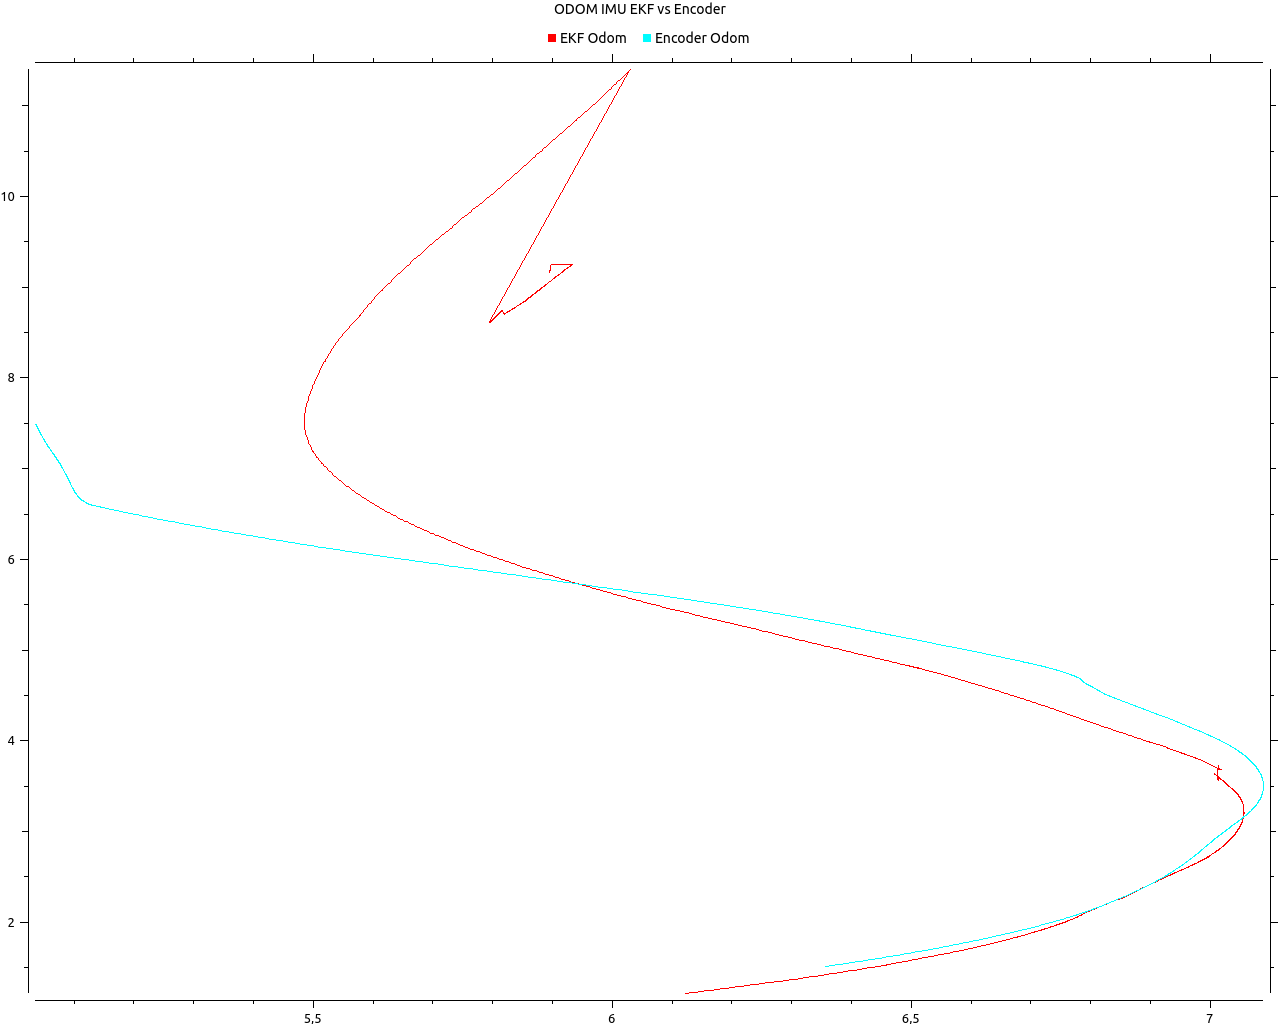
\includegraphics[width=\textwidth]{Pictures/odom pose comp}
	\caption{pose comparison wheel odom + IMU}
	\label{pose comparison wheel odom + IMU}

\end{figure}

\begin{figure}[H]
	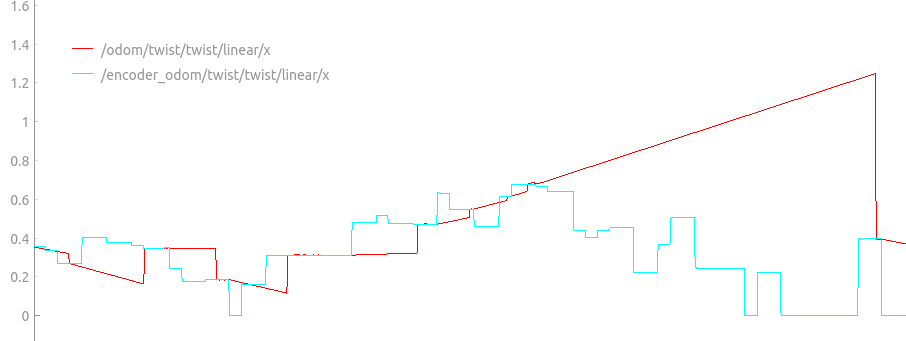
\includegraphics[width=\textwidth]{Pictures/comparison odom}
	\caption{velocity comparison wheel odom + IMU}
	\label{velocity comparison wheel odom + IMU}

\end{figure}


To fix this a logical approach is to include more data about the robots movement. Fortunately robot\_localization has an input for command velocities such as velocities produced by move base. While the command velocity does not provide any measurement in the real world the ekf filter can profit from knowing what the velocity actually should be.\\
It is very important to set the control timeout to a value that is larger than the cycle time of move\_base. Otherwise this will lead to translational offsets caused by too low estimate for the velocities like shown in Figure \ref{velwithcmd}.

\begin{figure}[H]
	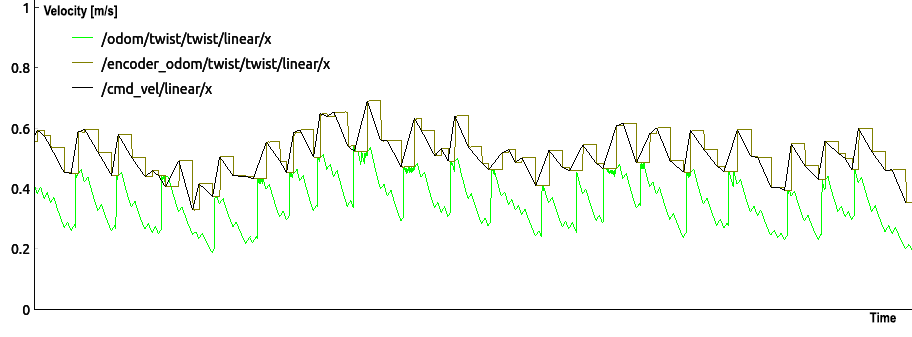
\includegraphics[width=\textwidth]{Pictures/velocity comp}
	\caption{velocity offset caused by too low control timout}
	\label{velocity offset}

\end{figure}


After the inclusion of the command velocity the acceleration limits in the configuration file of robot\_localization can be set equal to the limits in the local planner.

When observing both the pose and velocities again it is noticeable, that the odometry has drastically improved as pictured in Figure \ref{Odometry comparison wheel odomIMUcmdvel}, equally the velocities stay closer together as pictured in \ref{velwithcmd}.

\begin{figure}[H]
	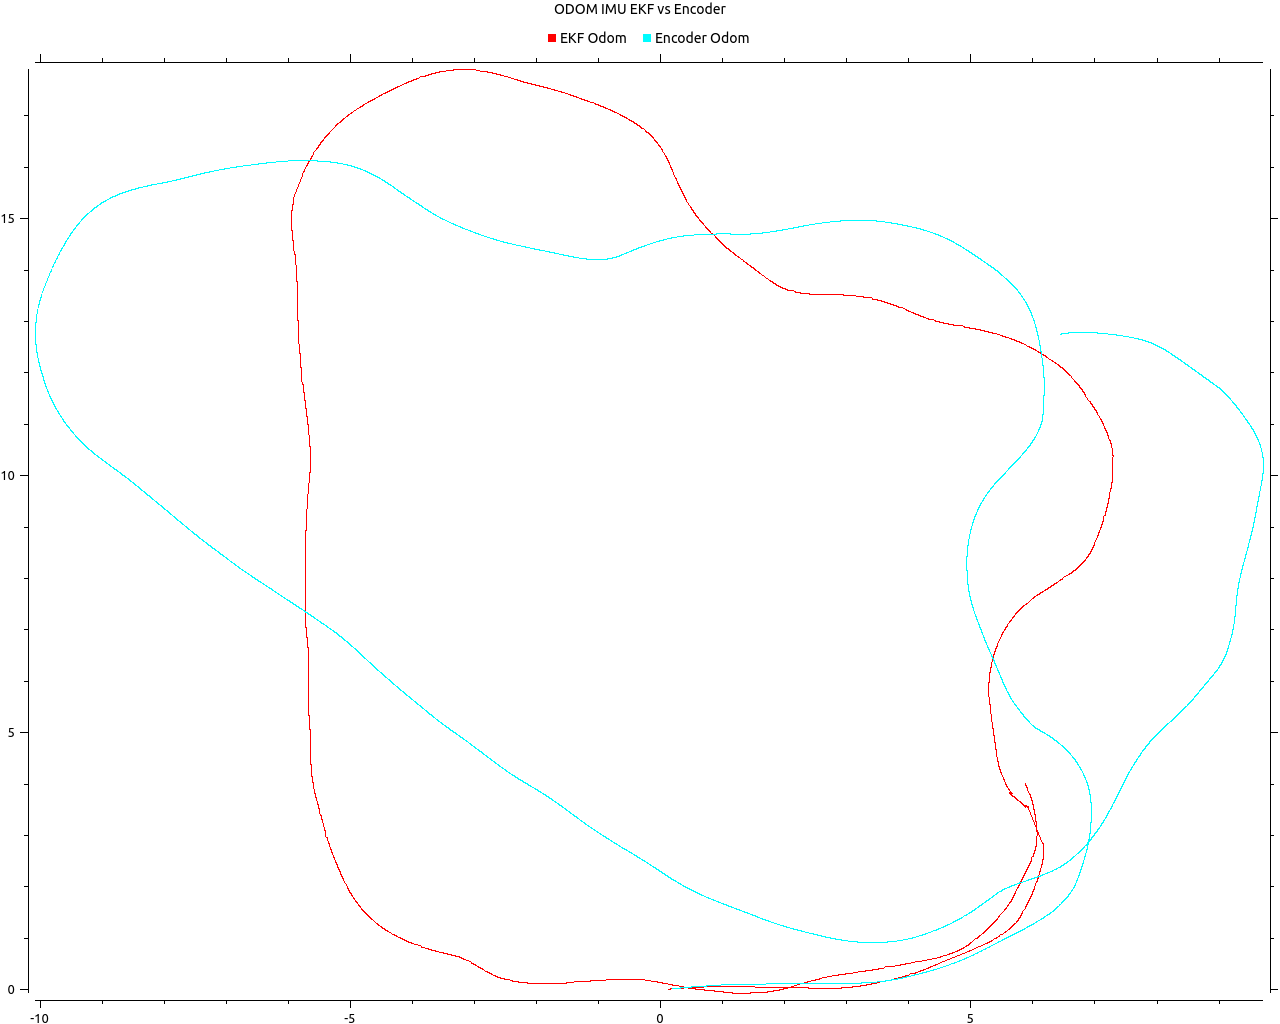
\includegraphics[width=\textwidth]{Pictures/odom after one round}
	\caption{Odometry comparison wheel odom + IMU + cmd\_vel}
	\label{Odometry comparison wheel odomIMUcmdvel}

\end{figure}
\begin{figure}[H]
	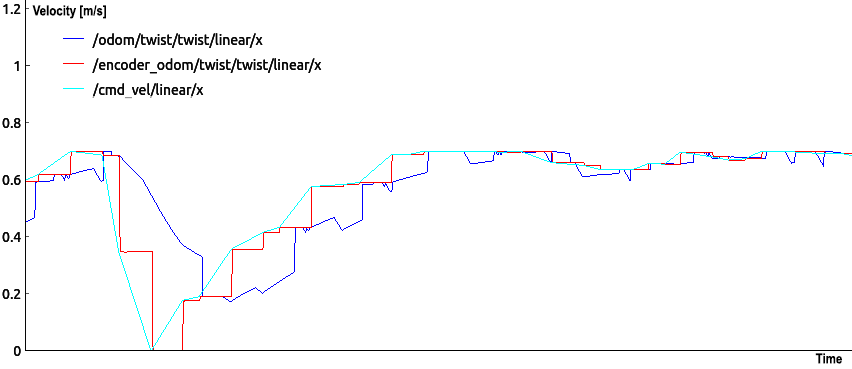
\includegraphics[width=\textwidth]{Pictures/circle vel}
	\caption{Velocity comparison with cmd\_vel}
	\label{velwithcmd}
\end{figure}



\begin{figure}[H]
	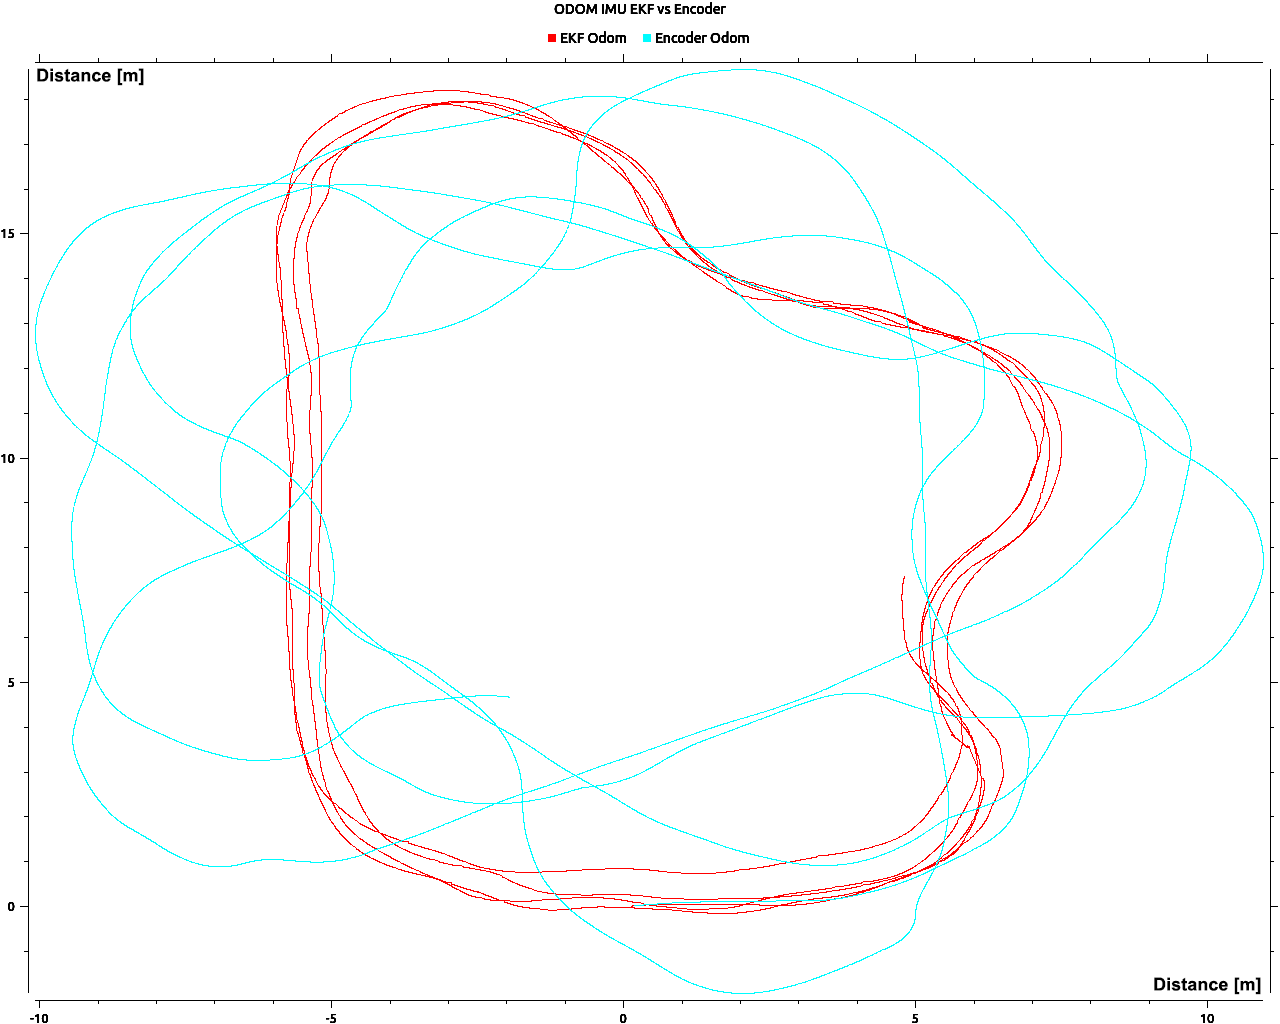
\includegraphics[width=\textwidth]{Pictures/odom comp multiple rounds}
	\caption{Odom comparison multiple rounds}
	\label{Odom comparison multiple rounds}

\end{figure}

Even after four rounds the odometry has not gained a large error in both translational and rotational as pictured in Figure \ref{Odom comparison multiple rounds}, furthermore the difference between the original odometry of the wheel encoders to the odometry from robot localization is quite remarkable.

After the rotantional and translational errors are marginal the scale of the odometry needs to be checked.
To isolate the different errors from the scaling error a circular track is build with a radius of 10 meter. Since the turning radius is constant this isolates the rotational error which can be seen at the graph of the wheel odometry in Figure \ref{circular track}.\\
The radius was chosen that high so potential errors are amplified and easier detectable.\\

Since the robot is driving on the lane and not on the middle road marking the expected radius is 10,45 meter. When evaluating the EKF odom in Figure \ref{circular track} we see that the scale is very precise.
 
\begin{figure}[H]
	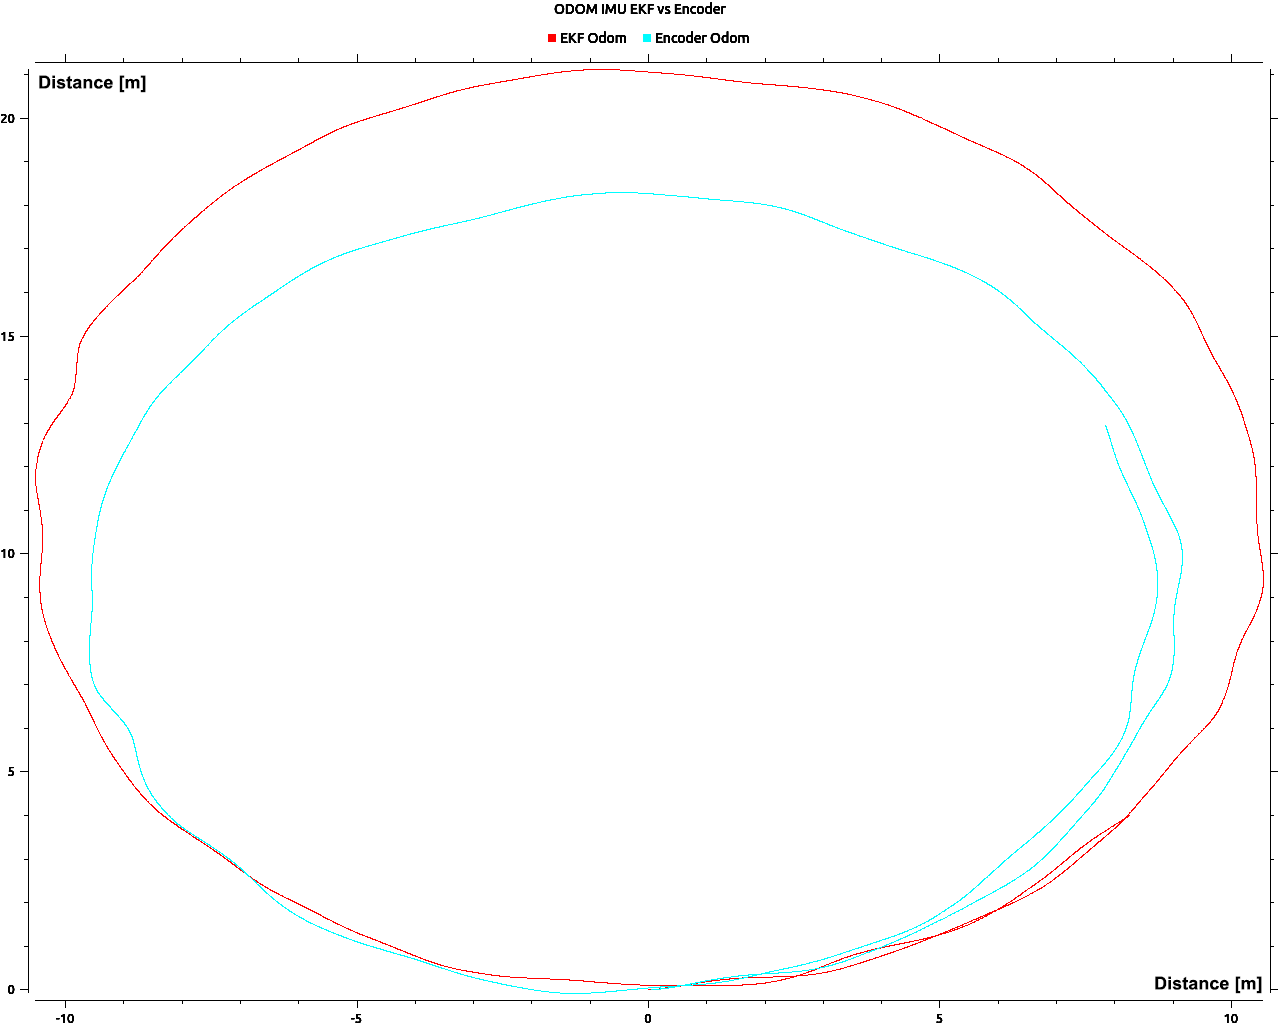
\includegraphics[width=\textwidth]{Pictures/circle odom}
	\caption{Odom comparison circular track}
	\label{circular track}

\end{figure}

As a final test the odometry from the robot\_localization node is compared to the true position from the simulation.

 \begin{figure}[H]
	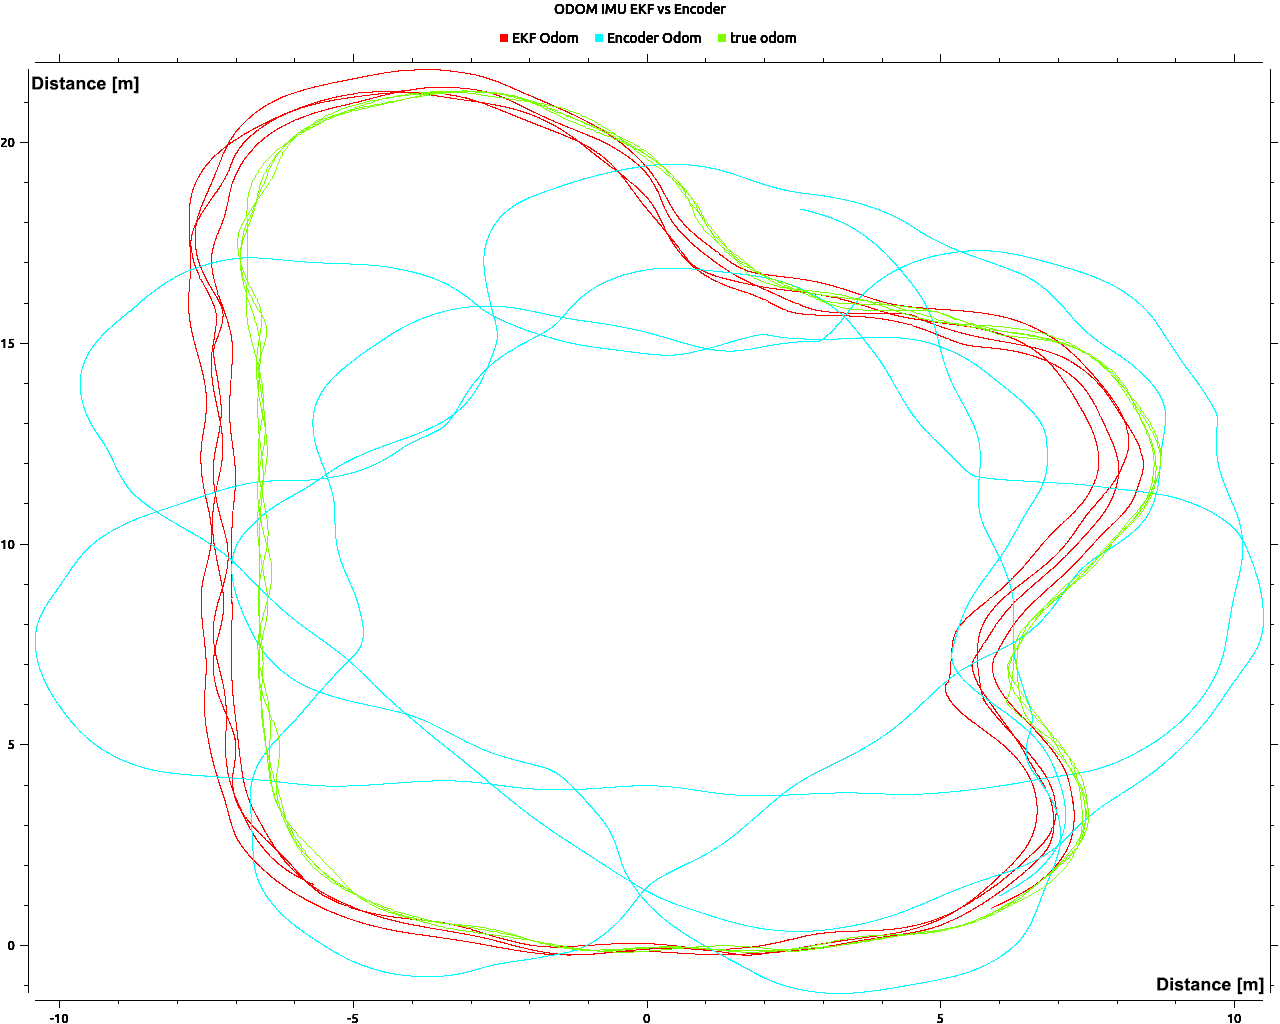
\includegraphics[width=\textwidth]{Pictures/odom with true}
	\caption{Comparison with true position}
	\label{trueodom}
\end{figure}

The comparison in Figure \ref{trueodom} shows, that the filtered odometry has a slight translational offset, but is very similar to the true odometry extracted from the simulation, hence it will be considered as sufficient for the navigation.


\section{Lidar test}


The Lidar sensor is simulated with realistic noise and errors. This also introduces the well known edge error in Laser distance measurement. 

When using a ``realistic'' lidar to project obstacles into the costmap this error produces a lot of lethal point like obstacles that significately hinder navigation as visible in Figure \ref{unfiltered lidar}.

\begin{figure}[H]
	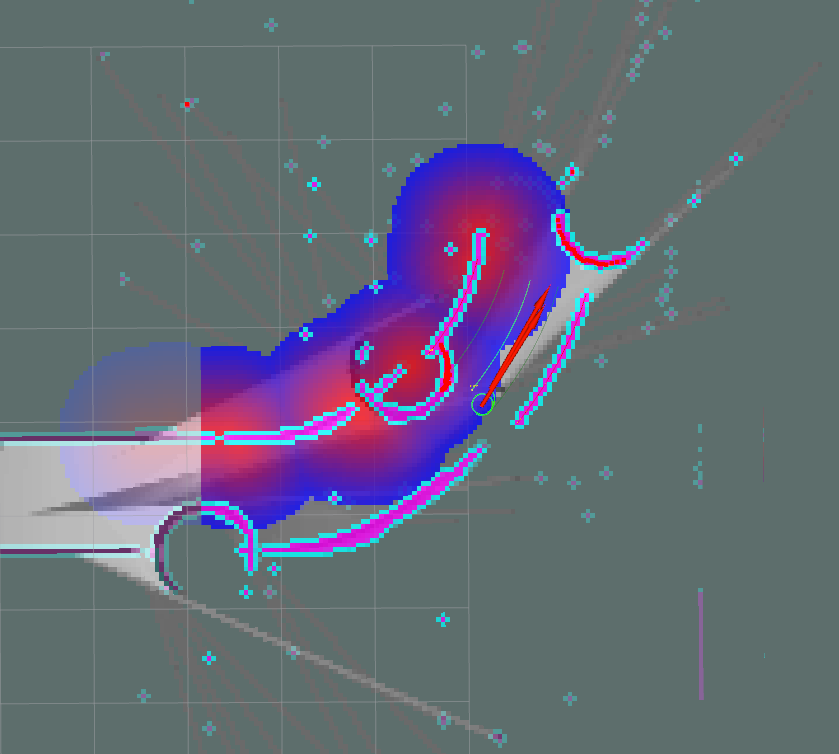
\includegraphics[width=\textwidth]{Pictures/Needs filtering of Laser}
	\caption{Lidar Test result}
	\label{unfiltered lidar}
\end{figure}

\subsection{Optimization}
To remove these error measurements the ROS package ``laser\_filters'' can be used. Among many different filter plugins that can be constructed into a filter chain it features the filter plugin ``ScanShadowFilter'' that is developed to remove the veiling effect around obstacles cause by the edge effect \cite{laserfilters}.


Figure \ref{lasercomp} shows a comparison between the filtered and not filtered laser scan, while keeping the data for 10 seconds. This allows to see the quickly jumping outliers caused by the edge effect. The filter seems well configured since the filtered points have no single outlier but still featuring a very good representation of the measured obstacle.

\begin{figure}[H]
	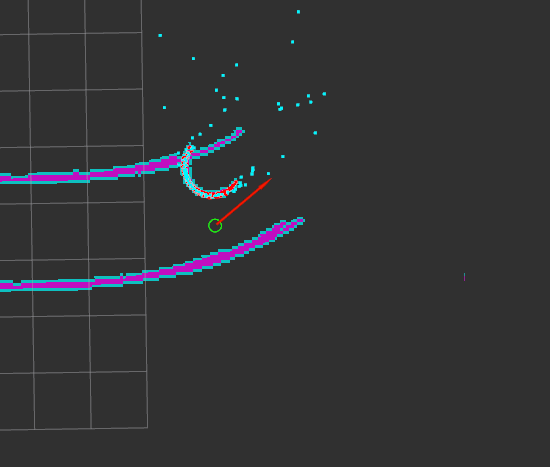
\includegraphics[width=\textwidth]{Pictures/LASERFILTER COMP}	
	\caption{comparison between filtered and not filtered laser scan (red - filtered, turquoise - raw)}
	\label{lasercomp}
\end{figure}

\section{road\_detection test}

As pictured in Figure \ref{longdurroad} the performance of the road detection converges to ca. 98.8\%. At the beginning the graph is not as reliable since there have not yet been enough measurements.\\

The duration of the test was roughly 1.5 hours of continuous navigation without obstacles in the simulation.

\begin{figure}[H]
	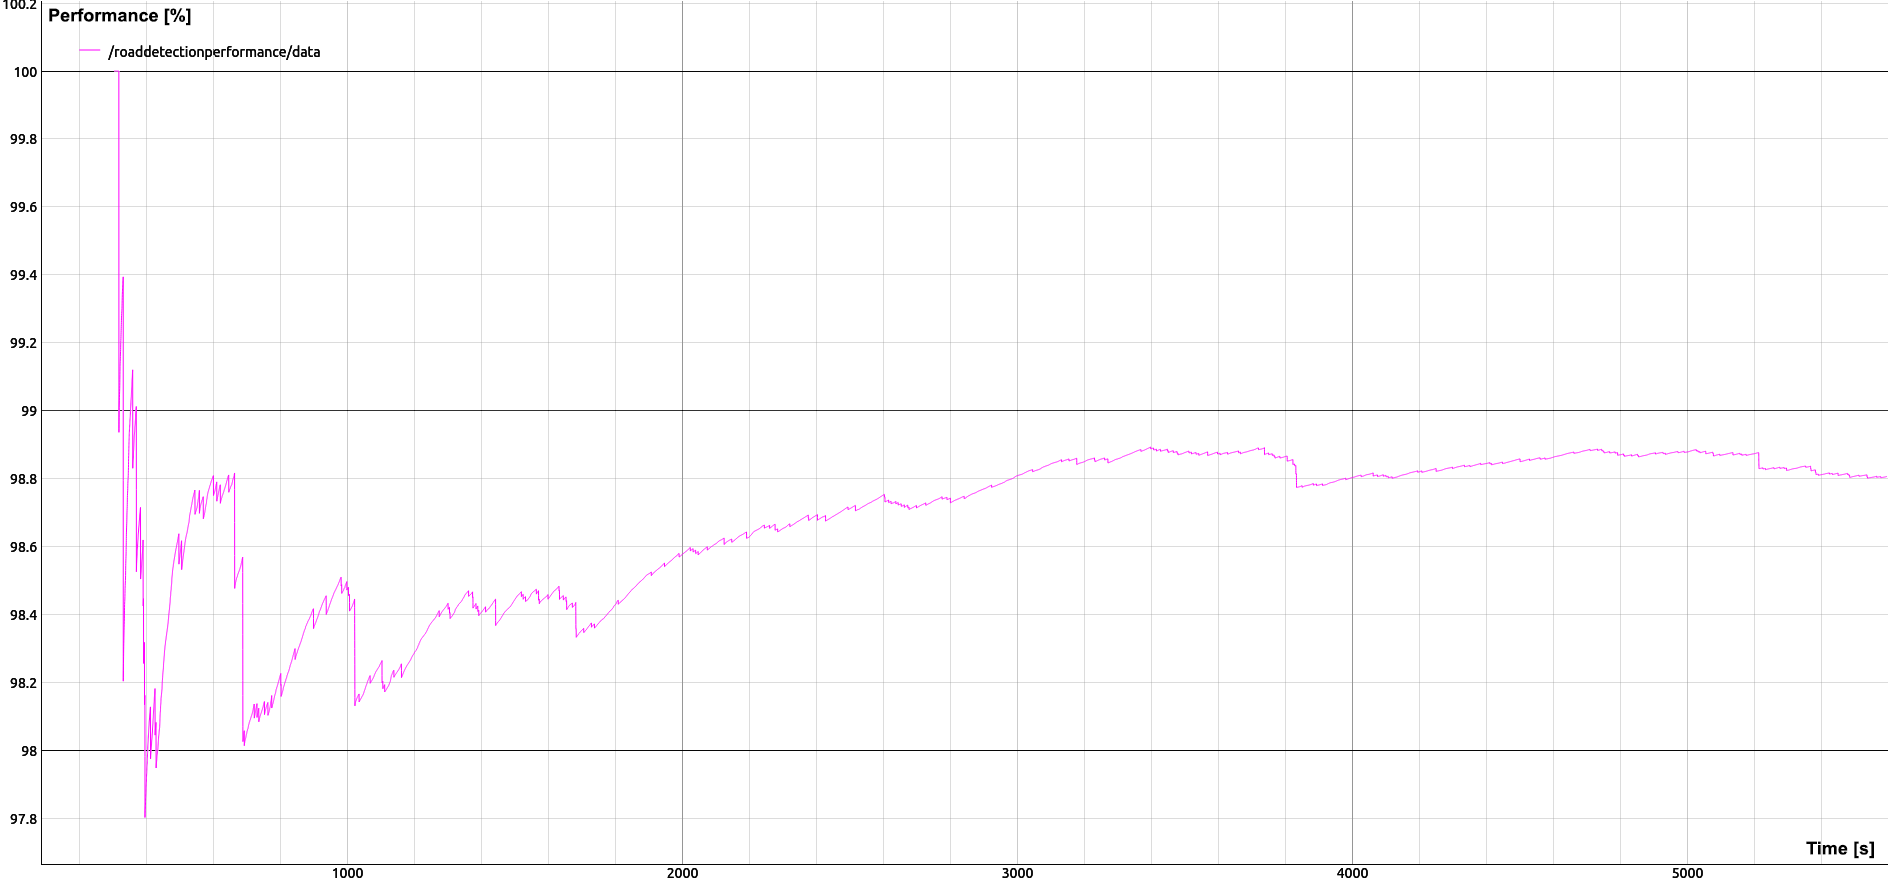
\includegraphics[width=\textwidth]{Pictures/long duration road detection test}
	\caption{roadRecordEvaluation during long duration test}
	\label{longdurroad}
\end{figure}

\section{SLAM test}
\textbf{Data purely from road detection:}\\

The following pictures contain the SLAM map after the \nth{1},\nth{2} and \nth{3} round.\\

\begin{figure}[H]
	\centering
	\begin{subfigure}{.3\linewidth}
		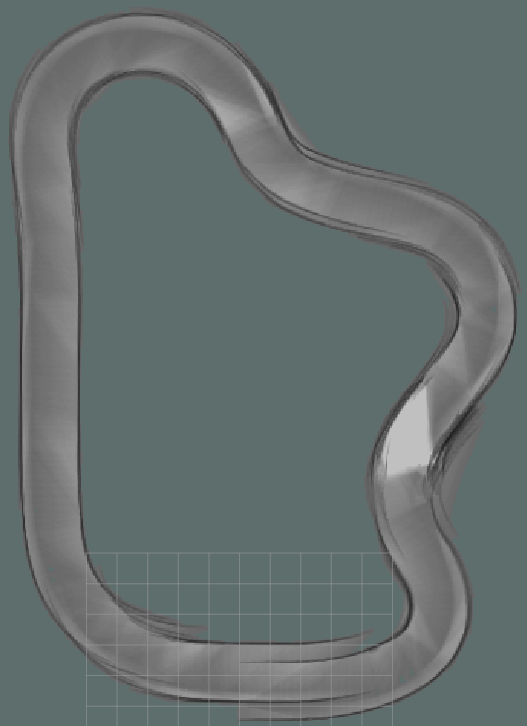
\includegraphics[width=\textwidth]{Pictures/1slamtest1}
		\caption{First}
		\end{subfigure}	
	%\hskip2em
	\begin{subfigure}{.3\linewidth}
		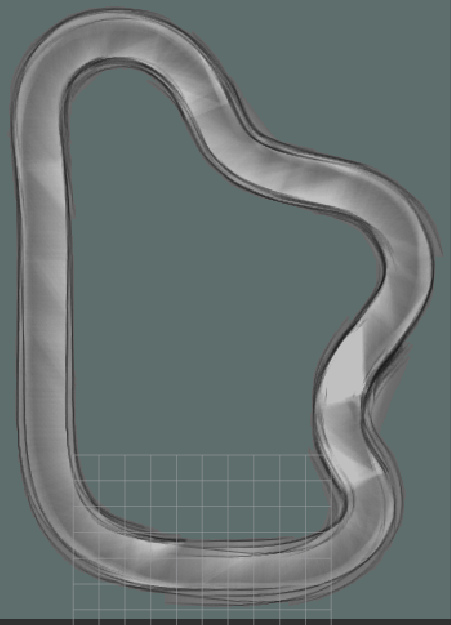
\includegraphics[width=\textwidth]{Pictures/1slamtest2}
		\caption{Second}
	\end{subfigure}
	%\hskip2em
	\begin{subfigure}{.3\linewidth}
		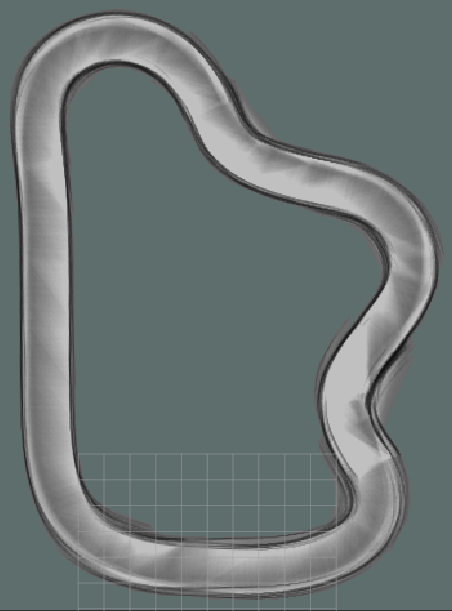
\includegraphics[width=\textwidth]{Pictures/1slamtest3}
		\caption{Third}
	\end{subfigure}

	\caption{Slam Map of first three rounds}
	\label{1slamtest}

\end{figure}

In the first round the map is not yet optimized. Like pictured in  Figure \ref{1slamtest} the road is not connected at the bottom after the first round, but has slight translational error.\\
In the second round the road is closed, but some submaps are slightly misaligned which can be seen by the blurry road markings.\\
This is well corrected in the third round and will improve from here on with every round, until the computational effort is too high.\\

\textbf{Data purely from localization and lidar scan with obstacles on the side of the road:}\\


As pictured in Figure \ref{2slamtest} cartographer manages to close the road already after the first round. After the second round the road borders are slightly blurry, therefore the submaps are not yet perfectly matched. This blurriness slightly improves after the third round, but the submaps are not yet perfectly matched with each other.

\begin{figure}[H]
	\centering
	\begin{subfigure}{.3\linewidth}
		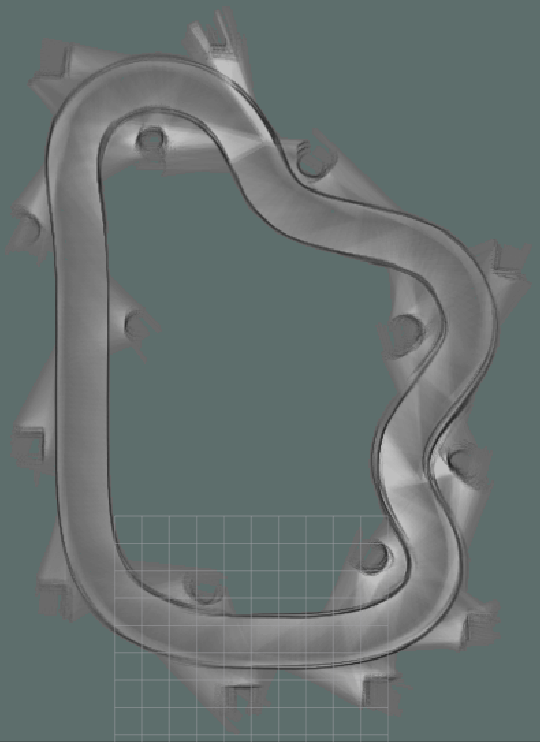
\includegraphics[width=\textwidth]{Pictures/2slamtest1}
		\caption{\nth{1} round}
		\end{subfigure}	
	%\hskip2em
	\begin{subfigure}{.3\linewidth}
		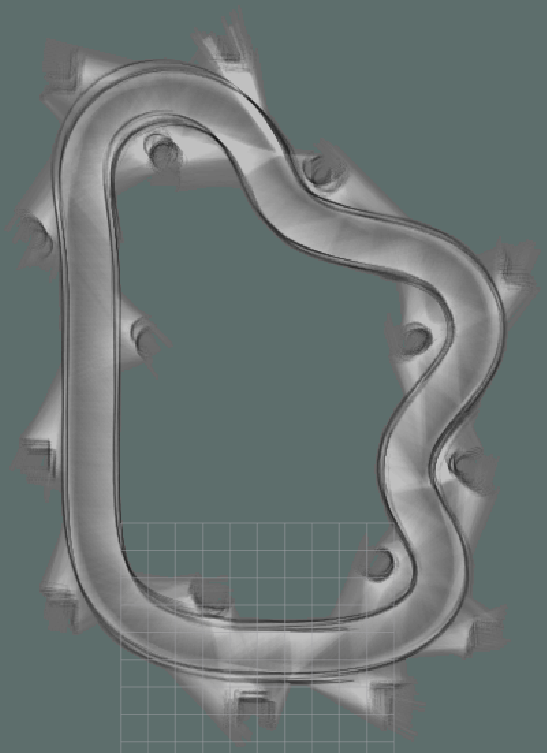
\includegraphics[width=\textwidth]{Pictures/2slamtest2}
		\caption{\nth{2} round}
	\end{subfigure}
	%\hskip2em
	\begin{subfigure}{.3\linewidth}
		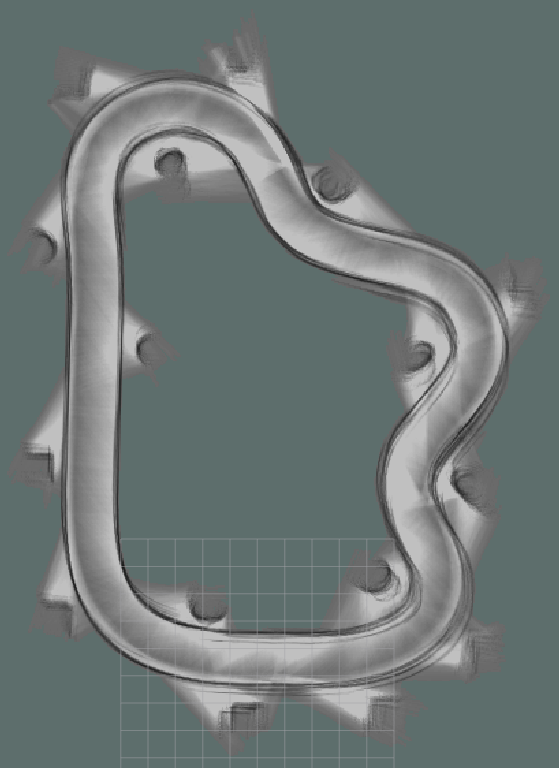
\includegraphics[width=\textwidth]{Pictures/2slamtest3}
		\caption{\nth{3} round}
	\end{subfigure}

	\caption{Slam Map of first three rounds}
	\label{2slamtest}

\end{figure}



\textbf{Long duration test with both road detection and lidar scan with obstacles on the side of the road:}\\

The map build by cartographer during this test (Figure \ref{3slamtest}) shows, that the map builds a very good representation of the real environment over the first four rounds.\\

After the \nth{7} round it is noticeable, that the matching of submaps seems to take more and more time, which is visible by a trace of unmatched submaps, that are slightly shifted. This is caused by the computational burden caused by the amount of submaps. In this round the cartographer node already takes up 20\% of the cpu resources and increases continuously. At this point realtime scan and submap matching is not possible anymore, resulting in enormous processing delays.

\begin{figure}[H]
	\centering
	\begin{subfigure}{.3\linewidth}
		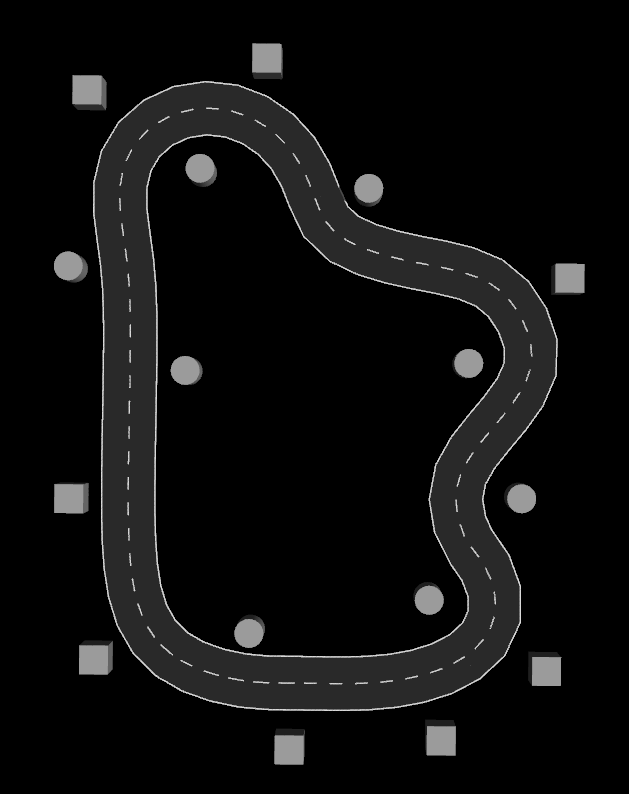
\includegraphics[width=\textwidth]{Pictures/2slamtest}
		\caption{Real Environment}
		\end{subfigure}	
	%\hskip2em
	\begin{subfigure}{.3\linewidth}
		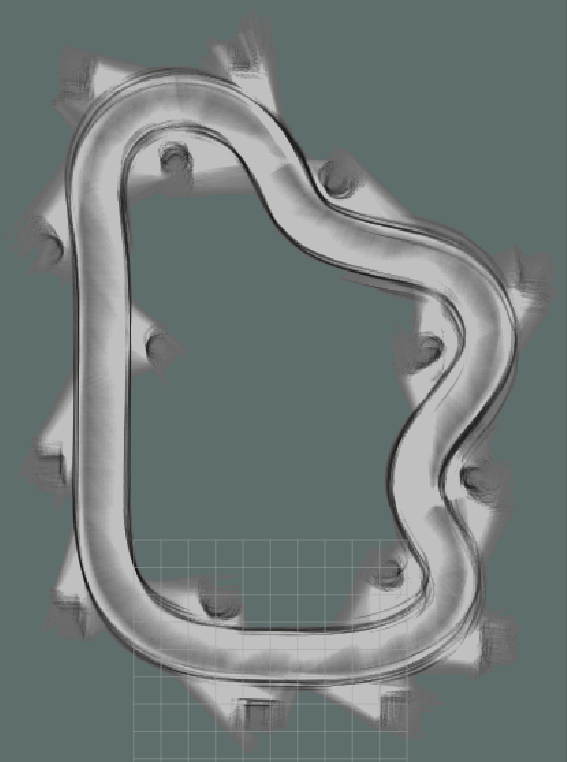
\includegraphics[width=\textwidth]{Pictures/2slamtest4}
		\caption{\nth{4} round}
	\end{subfigure}
	%\hskip2em
	\begin{subfigure}{.3\linewidth}
		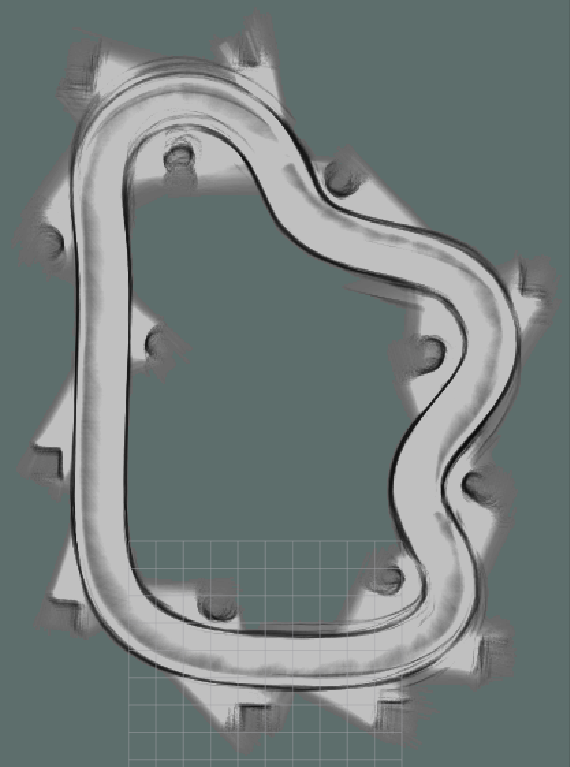
\includegraphics[width=\textwidth]{Pictures/2slamtest7}
		\caption{\nth{7} round}
	\end{subfigure}

	\caption{Slam Map rounds during long duration test}
	\label{3slamtest}

\end{figure}


\textbf{Data purely from localization and lidar scan with obstacles on the road:}\\

\begin{figure}[H]
	\centering
	\begin{subfigure}{.3\linewidth}
		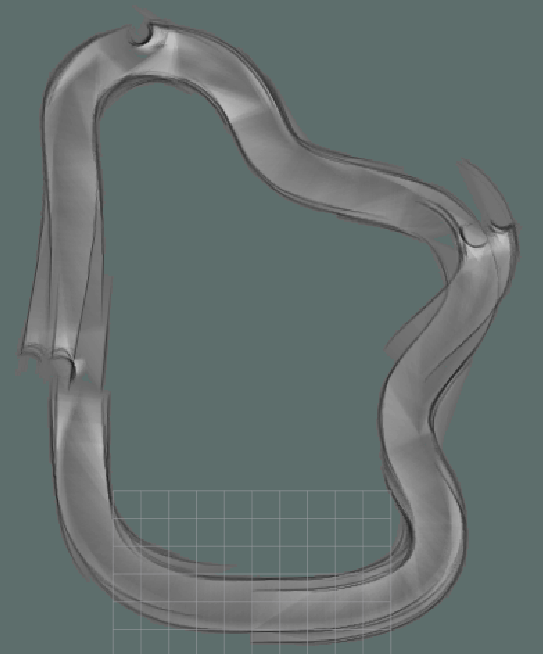
\includegraphics[width=\textwidth]{Pictures/3slamtest1}
		\caption{\nth{1} round}
		\end{subfigure}	
	%\hskip2em
	\begin{subfigure}{.3\linewidth}
		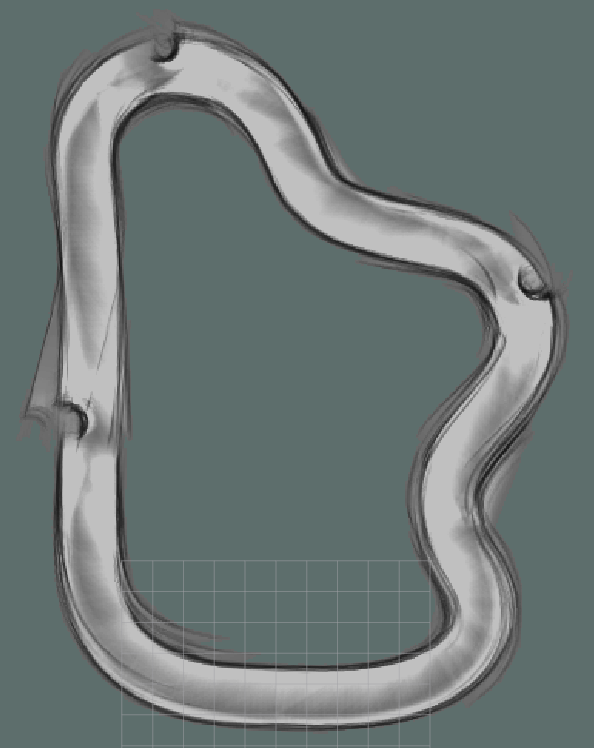
\includegraphics[width=\textwidth]{Pictures/3slamtest4}
		\caption{\nth{4} round}
	\end{subfigure}
	%\hskip2em
	\begin{subfigure}{.3\linewidth}
		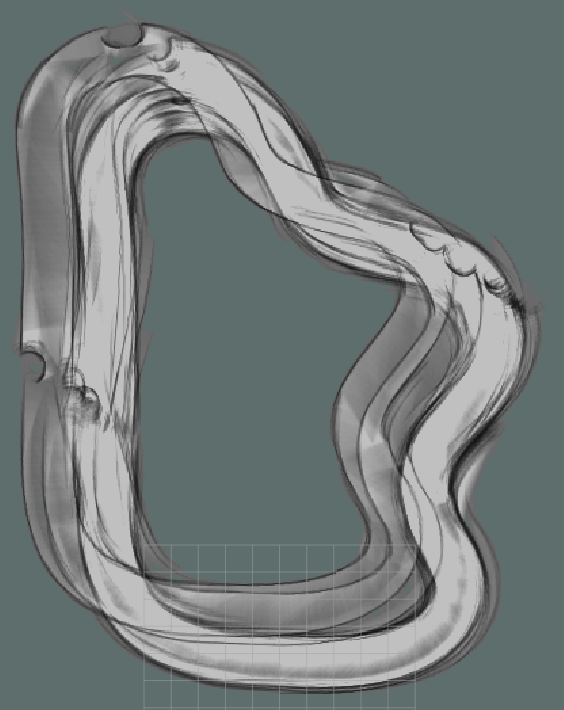
\includegraphics[width=\textwidth]{Pictures/3slamtest10}
		\caption{\nth{10} round}
	\end{subfigure}

	\caption{Slam Map rounds during long duration test}
	\label{4slamtest}

\end{figure}

As pictured in \ref{4slamtest} cartographer struggles with aligning the submaps during obstacle avoidance and suffers from rotational error.\\
Fortunately these errors are mostly corrected over the period of the next few rounds.\\ In the \nth{10} round however cartographer suffers from the same issue highlighted by the long duration test. Here it is clearly visible, that the queue of unmatched submaps is more than one entire round.\\

\textbf{Discussion of the test results}\\
As proven by the first two tests, cartographer is well tuned and the map would be useable for goal extraction. The submaps are well alligned and the map has no huge translational or rotational offset.\\

The \nth{3} and \nth{4} test on the other hand display the limitations of the slam algorithm in this use case.\\
When obstacles are located on the right lane the allignment of the submaps fails and a lot of submaps cant be attached to the rest of the map. After passing the same obstacle in multiple rounds the map improves to a point where it would be usable for goal extraction.\\
The \nth{3} test proves that cartographer is not usable in SLAM mode during long time navigation an a circuit. This is caused by the amount of submaps that are close to each other and the resulting amount of constraints between each of them.

Based on these test results it is not feasible to use the SLAM map for navigation with obstacles on the road, since the map is just not reliable enough and it is not certain of there are obstacles on the road or not. 




\section{complete system test}
The following subsections cover the discussion of the complete system tests.
\textbf{No obstacles}\\
The reasoning for this test is, to check how good the robot stays on the right lane. Therefore the robot drives in the described test environment, while the difference between the right lane and the robot center is monitored.

\begin{figure}[H]
	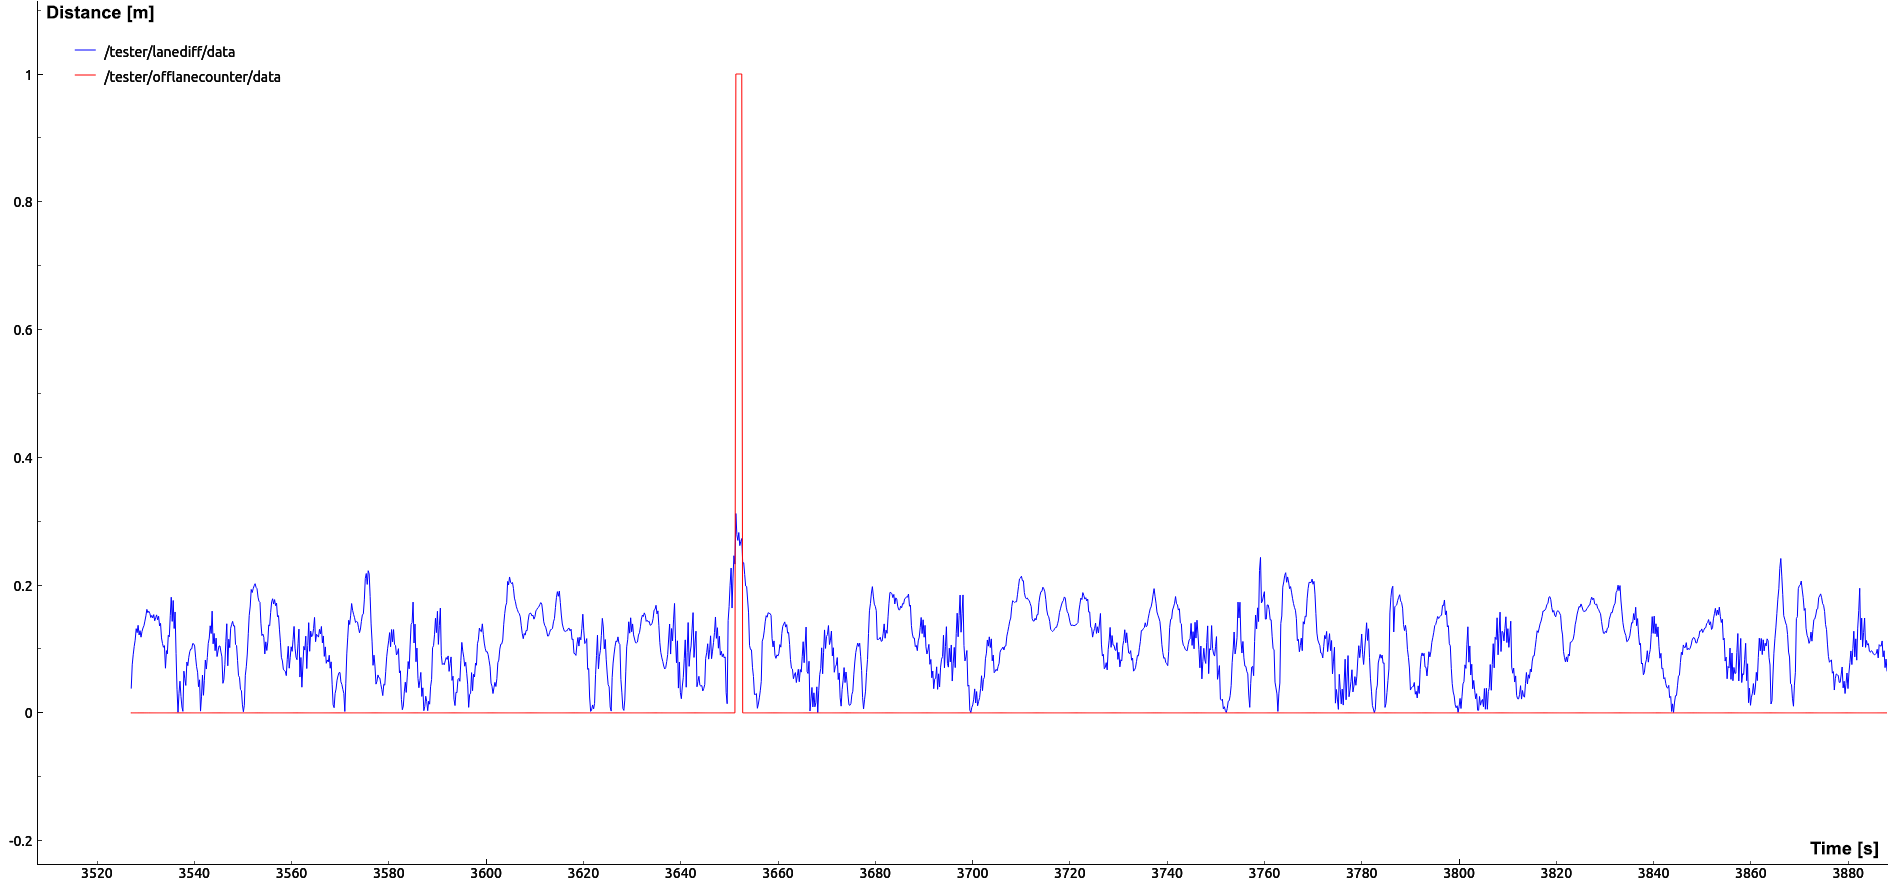
\includegraphics[width=\textwidth]{Pictures/final analysis no obstacle}
	\caption{absolute error of the robot trajectory and rectified signal of the avoidance duration}
	\label{noobserr}
\end{figure}

As pictured in \ref{noobserr} the robot has left the road markings once.\\

\begin{figure}[H]
	\begin{subfigure}{.5\linewidth}
		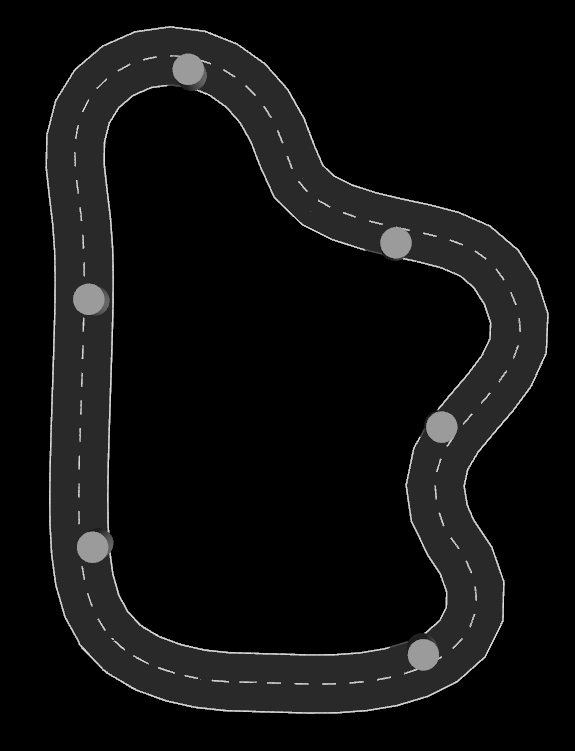
\includegraphics[width=\textwidth]{Pictures/obstacle left final 2}
		\caption{obstacles on left lane}
	\end{subfigure}	
	%\hskip2em
	\begin{subfigure}{.5\linewidth}
		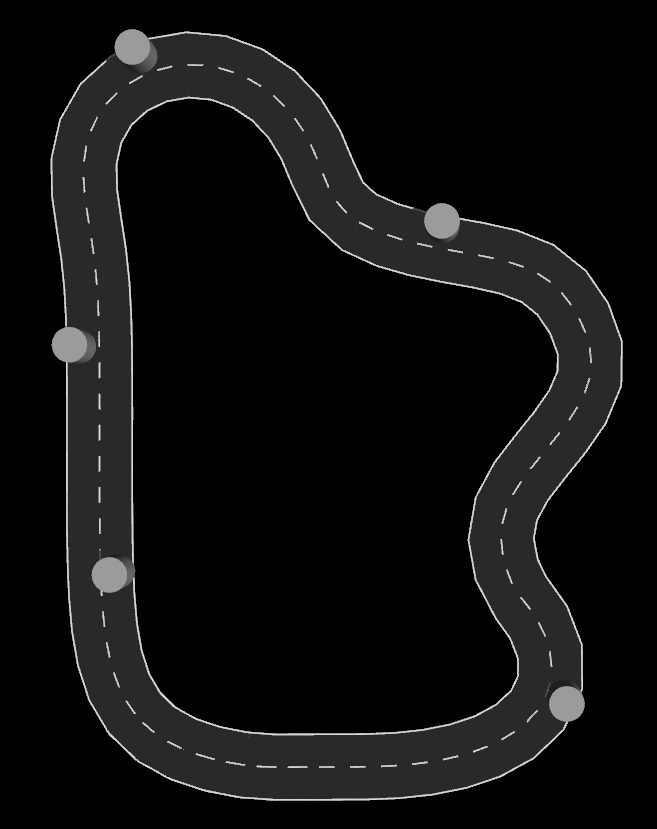
\includegraphics[width=\textwidth]{Pictures/right final obs}
		\caption{obstacles on right lane}
	\end{subfigure}

	\caption{Obstacle placement for both final tests}
	\label{obstaclefinaltest}

\end{figure}
\textbf{Obstacles on left lane}\\
This test is supposed to test the behavior of the navigation when obstacles block the view of the camera but the robot has to drive on the right side. In this test the robot will not drive as many rounds, since the goal is to observe the behavior when passing goals. In contrast to Figure \ref{noobserr} the distance to the nearest obstacle will be included in the graph, thus it can be determined, if the robot left the lane because it is near an obstacle or not, for this the true positions from the simulation will be used. The obstacle distance will only be tracked, if it is below 3 meters.
\begin{figure}[H]
	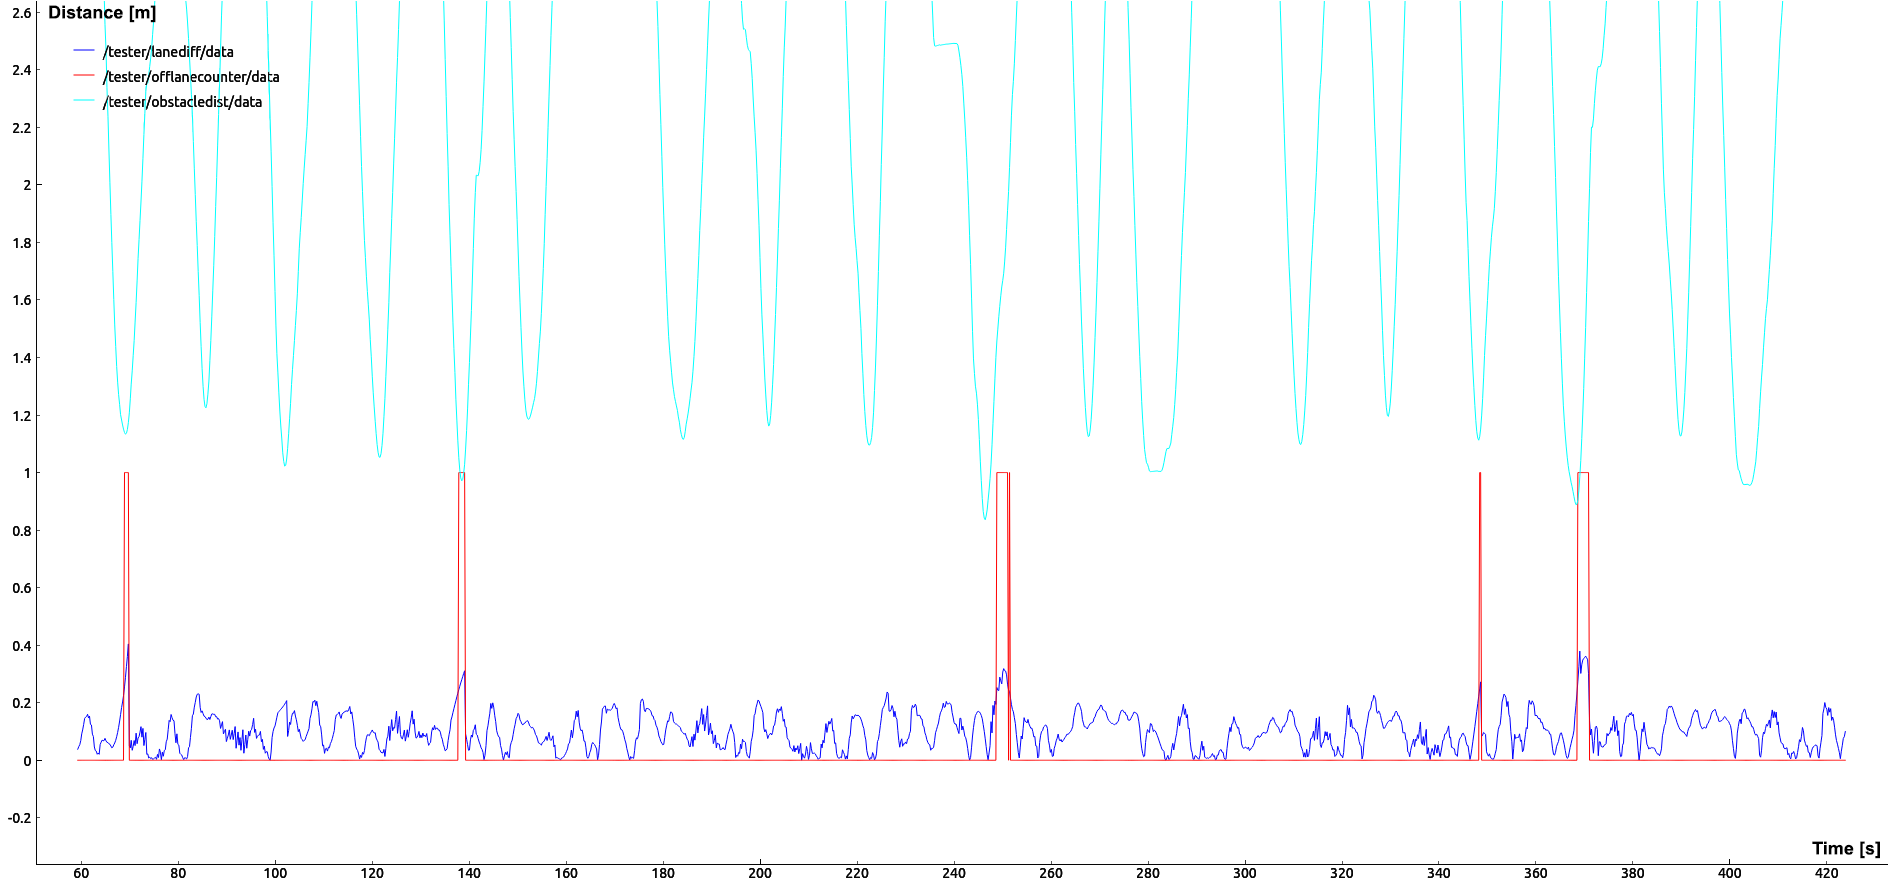
\includegraphics[width=\textwidth]{Pictures/left obs final obs2}
	\caption{graph of left lane obstacle test}
	\label{leftobsfinal}
\end{figure}
As visible in figure \ref{leftobsfinal} the robot left the right lane way more often compared to \ref{noobserr}.\\

\textbf{Obstacles on right lane}\\

To cover the possible scenarios of the carolo cup this test is supposed to be a realistic application with a few obstacle scattered over the entire environment on the right lane. Like in the last test the obstacles will be located as well in corners, as on straight sections of the road.

\begin{figure}[H]
	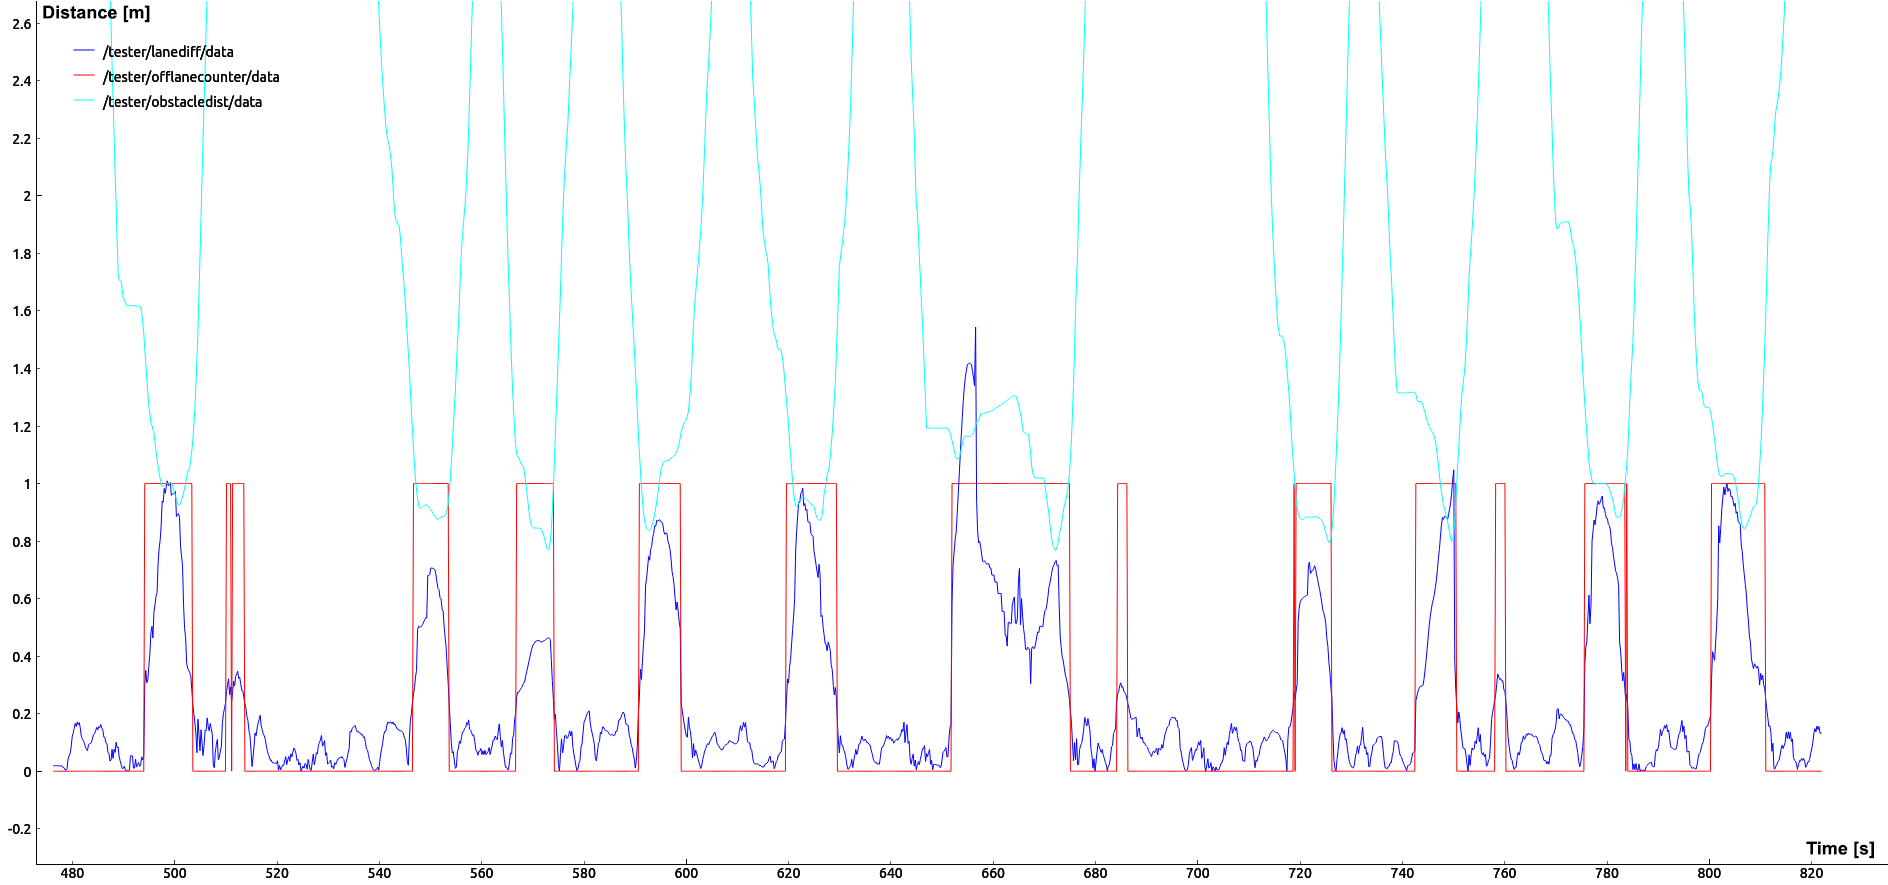
\includegraphics[width=\textwidth]{Pictures/right obs final obs}
	\caption{graph of right lane obstacle test}
	\label{rightobsfinal}
\end{figure}


As pictured in Figure \ref{obstaclefinaltest}, there are five obstacles on the right lane. These can be seen, when inspecting the graphe in Figure \ref{rightobsfinal}, which shows two rounds of the robot.

Furthermore the graph shows, that the robot successfully avoided all obstacles in both rounds. Unfortunately the robot left the lane three times, when no obstacle in the proximity of it.\\

In the middle of the graph the robot took particularly long for the avoidance.

The graph also shows, that the avoidance is all ways finished before the robot is two meters away from the obstacle and therefore satisfies this condition.

\subsection{Discussion}

The results of the complete system tests show, that the navigation performs really well during simple lane following, since the road detection recognizes the road almost allways as shown in the road\_detection test.

While observing the robot during driving past obstacles on the left lane it was noticeable, that the robot mostly left the lane, directly after it passed an obstacle in or directly after a corner.\\ 
In this case the predicted goal pulls the robot into the middle of the road, since the costmap does not yet have information about the road and therefore will not force the global plan to the right lane. The approximated goal is still constructed with the circle approximation since the upcoming straight section has net yet been seen.\\

Obstacle avoidance suffers from a similar problem. As shown in the \nth{3} test. Here it is visible, that the robot passes the obstacle nicely, but after passing drives along the center of the road, which causes the spikes of the rectified signal visible in \ref{rightobsfinal} after the ovoidance. As soon as the robot has passed an obstacle fully it drives straight to the predicted goal while waiting on new data from the road\_detection, which often causes unnecessary long avoidance periods.







\chapter{Conclusion}
\label{Conclusion}
The goal of this thesis was the configuration and development of a software stack that allows a mobile platform to drive autonomously in a road like environment, while avoiding obstacles and preferring the right lane.
This has been achieved by formulating a concept and implementing it using the navigation stack of ROS and various open source plugins and packages.
For the remaining tasks packages containing nodes have been developed using C++ which are configurable for different environments and robots. These packages are provided in a git repository hosted at the following url.\\

\url{https://github.com/Tristan9497/RoutePlanning}\\

The resulting navigation has been tested in a simulated environment as a complete stack, aswell as the individual nodes them selves.\\

Testing allowed to highlight the strengths and weaknesses of the concept, which can be used as the guideline for future work on the established structure. The developed concept was found to be working good, especially on empty road sections.\\

With an increasing amount of obstacles the amount of times where the camera sees the road markings decreases, which therefore causes the navigation to fail.


\section{Personal conclusion}







\chapter{Outlook}
\label{outlook}

This thesis highlighted existing problems in the established navigation concept, which should be resolved to score high results in the Carolo-Cup. This section will give proposals and ideas for future work on the current state of the navigation.\\

Using the structure of move\_base a custom local and global planner plugin can be developed and exchanged with the current plugins.\\

It could be very interesting to explore different path finding algorithms than the ones offered in the global\_planner plugin. At this point the development of a custom global planner might be able to perform better given the known use case.\\

Seeing the performance of the elastic band in the local planner used in this thesis a potential approach could be to move the task of lane following to the local planner, by deforming the elastic band directly with the polynomials of the road detection and weighting them individually.\\

To decrease the amount of times, where the navigation has to wait until it receives data from the road\_detection, the approximated shape of the road could be drawn into the costmap and overwritten by new incoming data of the road. This could be implemented into the dynamic\_cost\_layer that has been developed during this work.

The exploration of V-REP or its successor CoppeliaSim might be interesting with focus on the sensor plugins, especially with focus on distortion of the camera image.\\

During the research required in this work Nav2 for ROS2, which is currently in development seemed to offer many features, that are not included in the current navigation stack of ROS Noetic. As this thesis is focused on the development based on ROS Noetic this has not been explored yet. Nav2 features a new implementation of a costmap, that features filters usable to define keep-out or slow areas, that might be usable for a cleaner way to guide the robot on the right lane. Therefore further exploration of this might be beneficial.\\

As lidar based SLAM seemed to perform not ideal visual SLAM might offer more precision since the road markings might offer more informations for scan matching than the extracted polynomials. Furthermore functionality to detect, if a map is closed and of a reasonable quality might be usable to end the SLAM procedure, export the current map and using localization only to avoid the problem of the steadily increasing computational burden.


\listoffigures %Abbildungsverzeichnis

\listoftables %Tabellenverzeichnis

%\lstlistoflistings %Quelltextverzeichnis

%\printnomenclature %Abküzungsverzeichnis

\renewcommand{\bibname}{References}
\printbibliography


%ANHANG
\cleardoublepage
\pagenumbering{Roman} %Big romanian Pagenumbering
\setcounter{page}{1} %Seitenzähler zurücksetzen

\thispagestyle{plain}
\appendix %Anhang einfuegen


%TABLE OF CONTENTS APPENDIX
\phantomsection
\addcontentsline{toc}{chapter}{Appendix}
\startcontents[appendix]
\renewcommand\contentsname{\huge Appendix}% if a change of the default "Contents" name is required
\printcontents[appendix]{ }{0}{\section*{\contentsname}}
\stopcontents[main]
\newpage
%APPENDIX

\thispagestyle{empty}
\chapter{Additional Topics}
\label{AppendixAdditionalTopics}














\thispagestyle{empty}













\thispagestyle{empty}
\chapter{Organisation Chart}
\label{AppChart}

\begin{figure}[h!]
\begin{center}
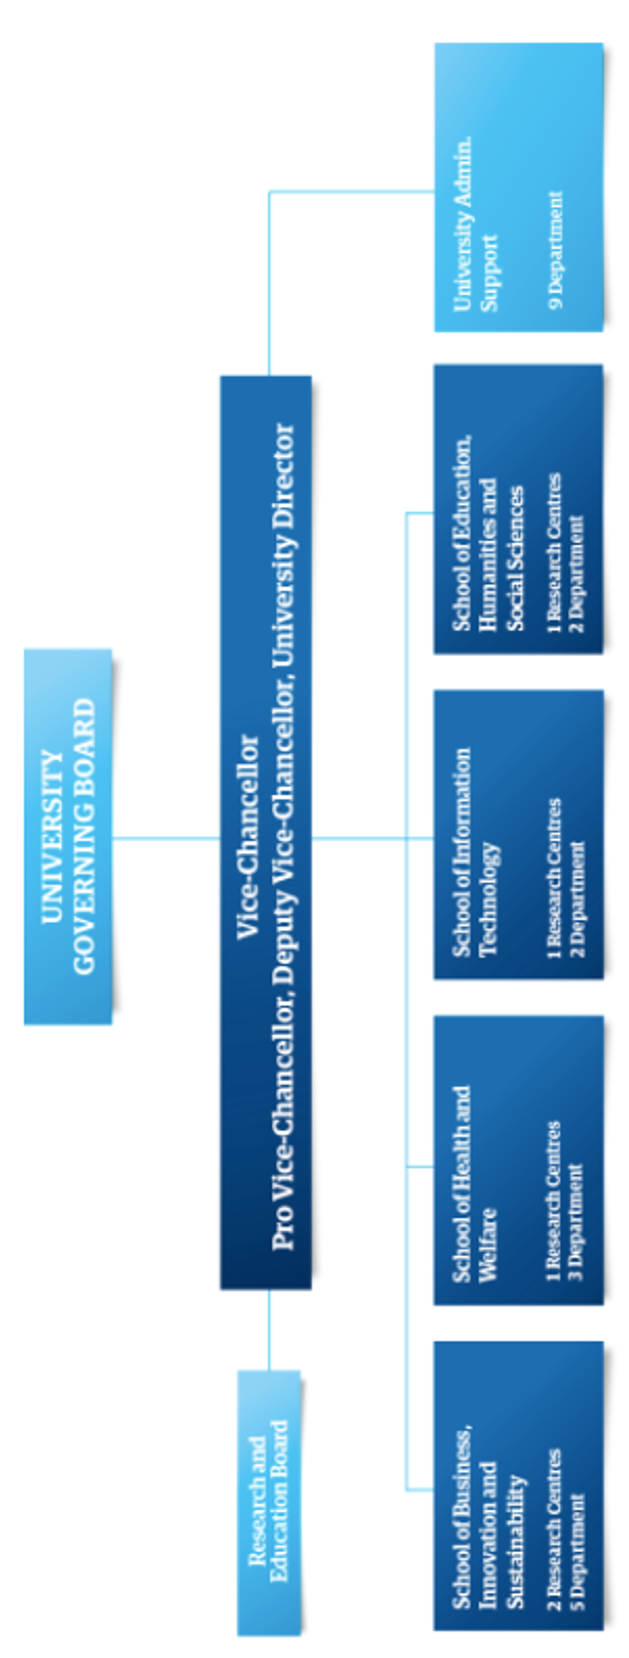
\includegraphics[width=7cm]{Pictures/AppChart}
\end{center}
\end{figure}

\thispagestyle{empty}
\chapter{Source Code}
\label{appendixSoureCode}



\stopcontents[appendix]

\begin{otherlanguage}{ngerman}
\addchap*{Eidesstattliche Erklärung}

\vspace*{5mm}

\thispagestyle{empty}

\begin{flushleft}
\begin{tabular}[h]{p{60mm}l p{60mm}l}
\textbf{Name:} Schwörer 			&\textbf{Vorname:} Tristan\\
\textbf{Matrikel-Nr.:} 71336		&\textbf{Studiengang:} Mechatronik\\
\end{tabular}
\end{flushleft}

\vspace*{11mm}

Hiermit versichere ich, \textbf{Tristan Schwörer}, an Eides statt, dass ich die vorliegende Bachelorarbeit

an der \textbf{Hochschule Aalen}

mit dem Titel \textbf{„Entwicklung von Navigationssoftware für mobile Robotersysteme und Simulation“}

selbständig und ohne fremde Hilfe verfasst und keine anderen als die angegebenen Hilfsmittel benutzt habe. Die Stellen der Arbeit, die dem Wortlaut oder dem Sinne nach anderen Werken entnommen wurden, sind in jedem Fall unter Angabe der Quelle kenntlich gemacht.\\

Ich habe die Bedeutung der eidesstattlichen Versicherung und prüfungsrechtlichen Folgen (\S 23 Abs. 3 des allg. Teils der Bachelor-SPO der Hochschule Aalen) sowie die strafrechtlichen Folgen (siehe unten) einer unrichtigen oder unvollständigen eidesstattlichen Versicherung zur Kenntnis genommen.\\

\vspace*{5mm}
\Large\textbf{Auszug aus dem Strafgesetzbuch (StGB)}


\normalsize\textbf{\S 156 StGB} Falsche Versicherung an Eides Statt

Wer von einer zur Abnahme einer Versicherung an Eides Statt zuständigen Behörde eine solche Versicherung falsch abgibt oder unter Berufung auf eine solche Versicherung falsch aussagt, wird mit Freiheitsstrafe bis zu drei Jahren oder mit Geldstrafe bestraft.

\vspace*{20mm}


\rule[-0.2cm]{5cm}{0.5pt} \hspace*{30mm}\rule[-0.2cm]{5cm}{0.5pt}
\newline
Ort, Datum\hspace*{61.85mm}Unterschrift

\end{otherlanguage} 


\end{document}
%%%%%%%%%%%%%%%%%%%%%%%%%%%%%%%%%%%%%%%%%%%%%%%%%%%%%%%%%%%%
%END_OF_FILE

















